%%%%%%%%%%%%%%%%%%%%%%%%%%%%%%%%%%%%%%%%%
% Compact Laboratory Book
% LaTeX Template
% Version 1.0 (4/6/12)
%
% This template has been downloaded from:
% http://www.LaTeXTemplates.com
%
% Original author:
% Joan Queralt Gil (http://phobos.xtec.cat/jqueralt) using the labbook class by
% Frank Kuster (http://www.ctan.org/tex-archive/macros/latex/contrib/labbook/)
%
% License:
% CC BY-NC-SA 3.0 (http://creativecommons.org/licenses/by-nc-sa/3.0/)
%
% Important note:
% This template requires the labbook.cls file to be in the same directory as the
% .tex file. The labbook.cls file provides the necessary structure to create the
% lab book.
%
% The \lipsum[#] commands throughout this template generate dummy text
% to fill the template out. These commands should all be removed when 
% writing lab book content.
%
% HOW TO USE THIS TEMPLATE 
% Each day in the lab consists of three main things:
%
% 1. LABDAY: The first thing to put is the \labday{} command with a date in 
% curly brackets, this will make a new section showing that you are working
% on a new day.
%
% 2. EXPERIMENT/SUBEXPERIMENT: Next you need to specify what 
% experiment(s) and subexperiment(s) you are working on with a 
% \experiment{} and \subexperiment{} commands with the experiment 
% shorthand in the curly brackets. The experiment shorthand is defined in the 
% 'DEFINITION OF EXPERIMENTS' section below, this means you can 
% say \experiment{pcr} and the actual text written to the PDF will be what 
% you set the 'pcr' experiment to be. If the experiment is a one off, you can 
% just write it in the bracket without creating a shorthand. Note: if you don't 
% want to have an experiment, just leave this out and it won't be printed.
%
% 3. CONTENT: Following the experiment is the content, i.e. what progress 
% you made on the experiment that day.
%
%%%%%%%%%%%%%%%%%%%%%%%%%%%%%%%%%%%%%%%%%

%----------------------------------------------------------------------------------------
%	PACKAGES AND OTHER DOCUMENT CONFIGURATIONS
%----------------------------------------------------------------------------------------                               

\documentclass[fontsize=11pt, % Document font size
                             paper=a4, % Document paper type
                             twoside, % Shifts odd pages to the left for easier reading when printed, can be changed to oneside
                             captions=tableheading,
                             index=totoc,
                             hyperref]{labbook}
 
\usepackage[bottom=10em]{geometry} % Reduces the whitespace at the bottom of the page so more text can fit

\usepackage[english]{babel} % English language
\usepackage{lipsum} % Used for inserting dummy 'Lorem ipsum' text into the template

\usepackage[utf8]{inputenc} % Uses the utf8 input encoding
\usepackage[T1]{fontenc} % Use 8-bit encoding that has 256 glyphs

\usepackage[osf]{mathpazo} % Palatino as the main font
\linespread{1.05}\selectfont % Palatino needs some extra spacing, here 5% extra
\usepackage[scaled=.88]{beramono} % Bera-Monospace
%\usepackage[scaled=.86]{berasans} % Bera Sans-Serif
\usepackage[rm,light]{roboto} % Roboto

\usepackage{booktabs,array} % Packages for tables

\usepackage{amsmath} % For typesetting math
\usepackage{graphicx} % Required for including images
\usepackage{etoolbox}
\usepackage[norule]{footmisc} % Removes the horizontal rule from footnotes
\usepackage{lastpage} % Counts the number of pages of the document

\usepackage[dvipsnames]{xcolor}  % Allows the definition of hex colors
\definecolor{titleblue}{rgb}{0.16,0.24,0.64} % Custom color for the title on the title page
\definecolor{linkcolor}{rgb}{0,0,0.42} % Custom color for links - dark blue at the moment

\addtokomafont{title}{\Huge\color{titleblue}} % Titles in custom blue color
\addtokomafont{chapter}{\color{OliveGreen}} % Lab dates in olive green
\addtokomafont{section}{\color{Sepia}} % Sections in sepia
\addtokomafont{pagehead}{\normalfont\sffamily\color{gray}} % Header text in gray and sans serif
\addtokomafont{caption}{\footnotesize\itshape} % Small italic font size for captions
\addtokomafont{captionlabel}{\upshape\bfseries} % Bold for caption labels
\addtokomafont{descriptionlabel}{\rmfamily}
\setcapwidth[r]{10cm} % Right align caption text
\setkomafont{footnote}{\sffamily} % Footnotes in sans serif

\deffootnote[4cm]{4cm}{1em}{\textsuperscript{\thefootnotemark}} % Indent footnotes to line up with text

\DeclareFixedFont{\textcap}{T1}{phv}{bx}{n}{1.5cm} % Font for main title: Helvetica 1.5 cm
\DeclareFixedFont{\textaut}{T1}{phv}{bx}{n}{0.8cm} % Font for author name: Helvetica 0.8 cm

\usepackage[nouppercase,headsepline]{scrpage2} % Provides headers and footers configuration
\pagestyle{scrheadings} % Print the headers and footers on all pages
\clearscrheadfoot % Clean old definitions if they exist

\automark[chapter]{chapter}
\ohead{\headmark} % Prints outer header

\setlength{\headheight}{25pt} % Makes the header take up a bit of extra space for aesthetics
\setheadsepline{.4pt} % Creates a thin rule under the header
\addtokomafont{headsepline}{\color{lightgray}} % Colors the rule under the header light gray

\ofoot[\normalfont\normalcolor{\thepage\ |\  \pageref{LastPage}}]{\normalfont\normalcolor{\thepage\ |\  \pageref{LastPage}}} % Creates an outer footer of: "current page | total pages"

% These lines make it so each new lab day directly follows the previous one i.e. does not start on a new page - comment them out to separate lab days on new pages
\makeatletter
\patchcmd{\addchap}{\if@openright\cleardoublepage\else\clearpage\fi}{\par}{}{}
\makeatother
\renewcommand*{\chapterpagestyle}{scrheadings}

% These lines make it so every figure and equation in the document is numbered consecutively rather than restarting at 1 for each lab day - comment them out to remove this behavior
\usepackage{chngcntr}
\counterwithout{figure}{labday}
\counterwithout{equation}{labday}

% Hyperlink configuration
\usepackage[
    pdfauthor={}, % Your name for the author field in the PDF
    pdftitle={Laboratory Journal}, % PDF title
    pdfsubject={}, % PDF subject
    bookmarksopen=true,
    linktocpage=true,
    urlcolor=linkcolor, % Color of URLs
    citecolor=linkcolor, % Color of citations
    linkcolor=linkcolor, % Color of links to other pages/figures
    backref=page,
    pdfpagelabels=true,
    plainpages=false,
    colorlinks=true, % Turn off all coloring by changing this to false
    bookmarks=true,
    pdfview=FitB]{hyperref}

\usepackage[stretch=10]{microtype} % Slightly tweak font spacing for aesthetics

%\setlength\parindent{0pt} % Uncomment to remove all indentation from paragraphs

%----------------------------------------------------------------------------------------
%	DEFINITION OF EXPERIMENTS
%----------------------------------------------------------------------------------------

% Template: \newexperiment{<abbrev>}[<short form>]{<long form>}
% <abbrev> is the reference to use later in the .tex file in \experiment{}, the <short form> is only used in the table of contents and running title - it is optional, <long form> is what is printed in the lab book itself

\newexperiment{example}[Example experiment]{This is an example experiment}
\newexperiment{example2}[Example experiment 2]{This is another example experiment}
\newexperiment{example3}[Example experiment 3]{This is yet another example experiment}

\newsubexperiment{subexp_example}[Example sub-experiment]{This is an example sub-experiment}
\newsubexperiment{subexp_example2}[Example sub-experiment 2]{This is another example sub-experiment}
\newsubexperiment{subexp_example3}[Example sub-experiment 3]{This is yet another example sub-experiment}

%----------------------------------------------------------------------------------------

\begin{document}

%----------------------------------------------------------------------------------------
%	TITLE PAGE
%----------------------------------------------------------------------------------------

\title{\textcap{Salton Sea Modeling Journal \\[1cm]  
\textaut{Beginning Jan-08-2015}}}

\author{
    \textaut{Valerie Sahakian}\\ \\ % Your name
     % Your degree
}
\date{} % No date by default, add \today if you wish to include the publication date

\maketitle % Title page

\printindex
\tableofcontents % Table of contents
\newpage % Start lab look on a new page

\begin{addmargin}[4cm]{0cm} % Makes the text width much shorter for a compact look

\pagestyle{scrheadings} % Begin using headers

%----------------------------------------------------------------------------------------
%	LAB BOOK CONTENTS
%----------------------------------------------------------------------------------------

\labday{Thursday, 8 January 2015}



%-----------------------------------------

\experiment{Modeling varying interfaces for the SSAF}

Try various surface expressions of the high-velocity interface to investigate how well-constrained this is, and if the interface is more likely to be to the East or West of the SSAF surface trace.  This will aid in determining what fault structure is present; if the fault is to the west of the surface trace of the SSAF, it is more likely a normal fault in the Salton Sea, not visible on land.  If it intersects the surface trace, it is likely that the fault may have a westward dip/oblique component; if to the east, there may be a larger normal fault cross-cutting the modern-day SSAF.

To modify the starting model and adjust the interface's surface trace, use the script:

/Modeling/salton\_line7base/vm/line7tomographymodels\_

/salton7base\_manip2.m

\subexperiment{Last time...Inversions 11, 12, and 13}

In October, inversions 12 and 13 were run; it turns out the "final" model I had before did not include constraints on the interface from the MCS reflector picks.  Inversions 12, and the final (13) were to correct this.  

\begin{figure}[h!]
\raggedleft
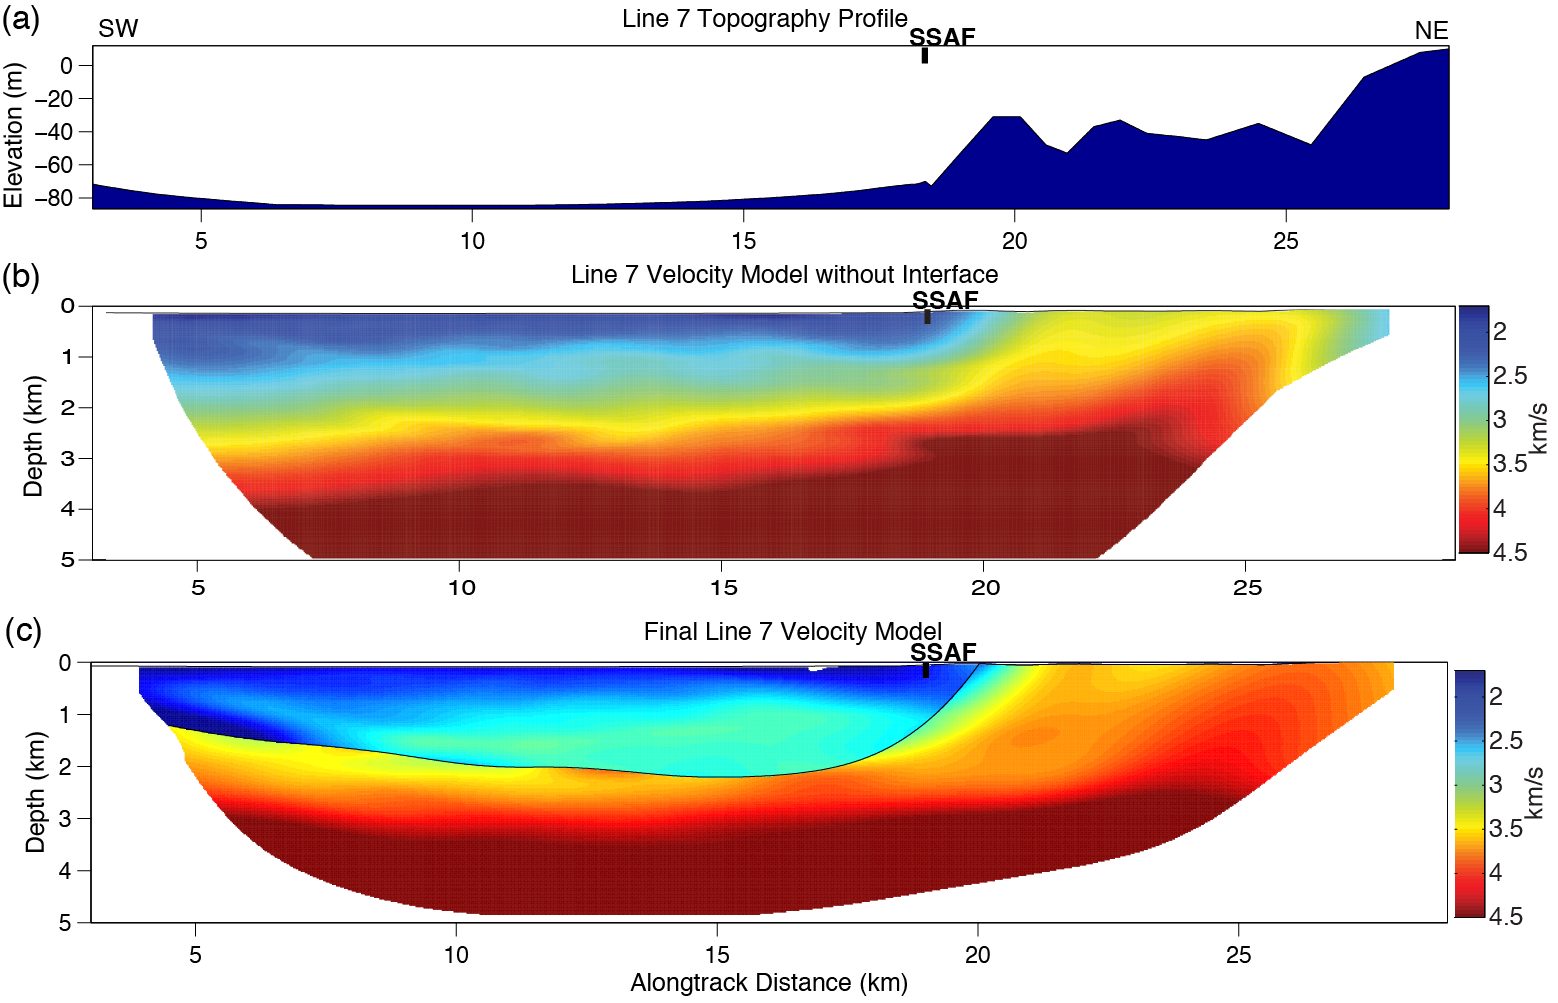
\includegraphics[scale=0.5,keepaspectratio=true]{figs/Salton7base_final11_topo_edit2.png}
\caption{Inversion 11 final model, without MCS constraints. (a) shows a topography profile; (b) shows the model without an interface; (c) shows the final model, with no MCS constraints, and with an interface.   Chi sq = 1.3.  }
\label{fig:line7noMCS}
\end{figure}

Inversions 12 and 13 were run with MCS constraints; the final model had a poorer chi sq than the other model; the question was why.  The best misfit came from inversion iteration 21, raytracing iteration 22, after applying the nullspace shuttles method.  This chi sq was 1.88, whereas without the MCS data it's 1.3.  The differences between the two are not that great, but with the MCS constraints the model looks a little splotchier because of where the layer 1 rays are turning.  The original final model, from inversion 11, can be seen in figure \autoref{fig:line7noMCS}; the final model with MCS constraints is seen in \autoref{fig:line7MCS}.  


\begin{figure}[h!]
\raggedleft
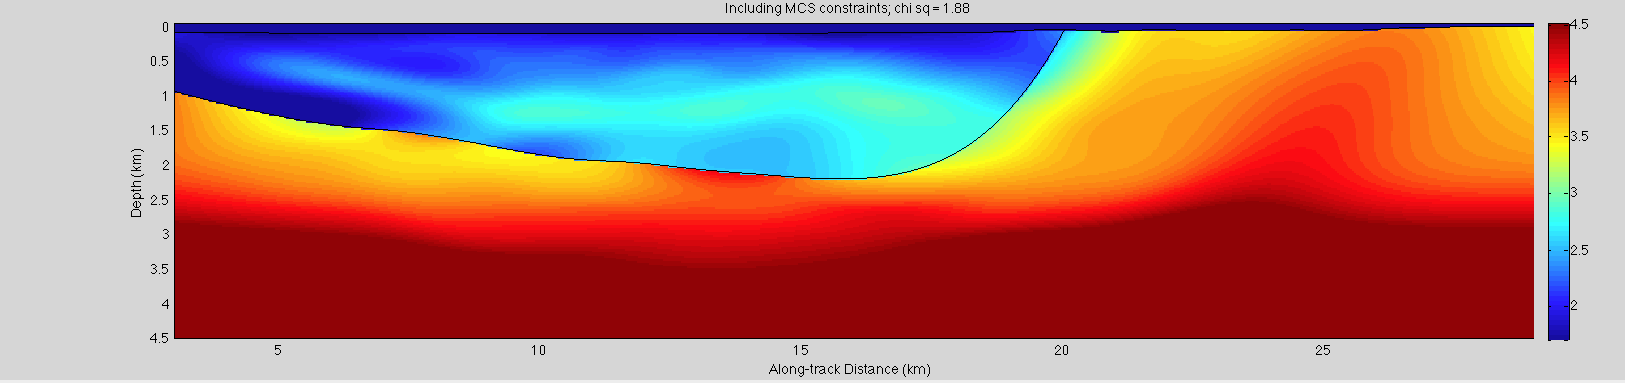
\includegraphics[scale=0.3,keepaspectratio=true]{figs/Line7_withMCS.png}
\caption{Inversion 13 final model, with MCS constraints.  Chi sq = 1.88.}
\label{fig:line7MCS}
\end{figure}

Alistair suggested looking at the reflection residuals:  

"I would look at how well, or not, the prediction of the previous model simply fits the trend in MCS reflection times, i.e. does it predict an increase in reflections times at about the same rate as seen in the MCS data?  If it does then it is possible that the is mostly a static time shift in your MCS picks relative to the OBS times.  If the trends aren't really compatible then you probably are doing about as well as you can in reconciling the different data within an single model.  and we should probably reconsider the possibility of the MCS reflections transgressing velocity contours."

To determine if this higher misfit is due to a consistently offset reflector, I plotted the just the reflection ray paths of the model with MCS constraints (\autoref{fig:line7MCS-resid}).   

\begin{figure}[h!]
\raggedleft
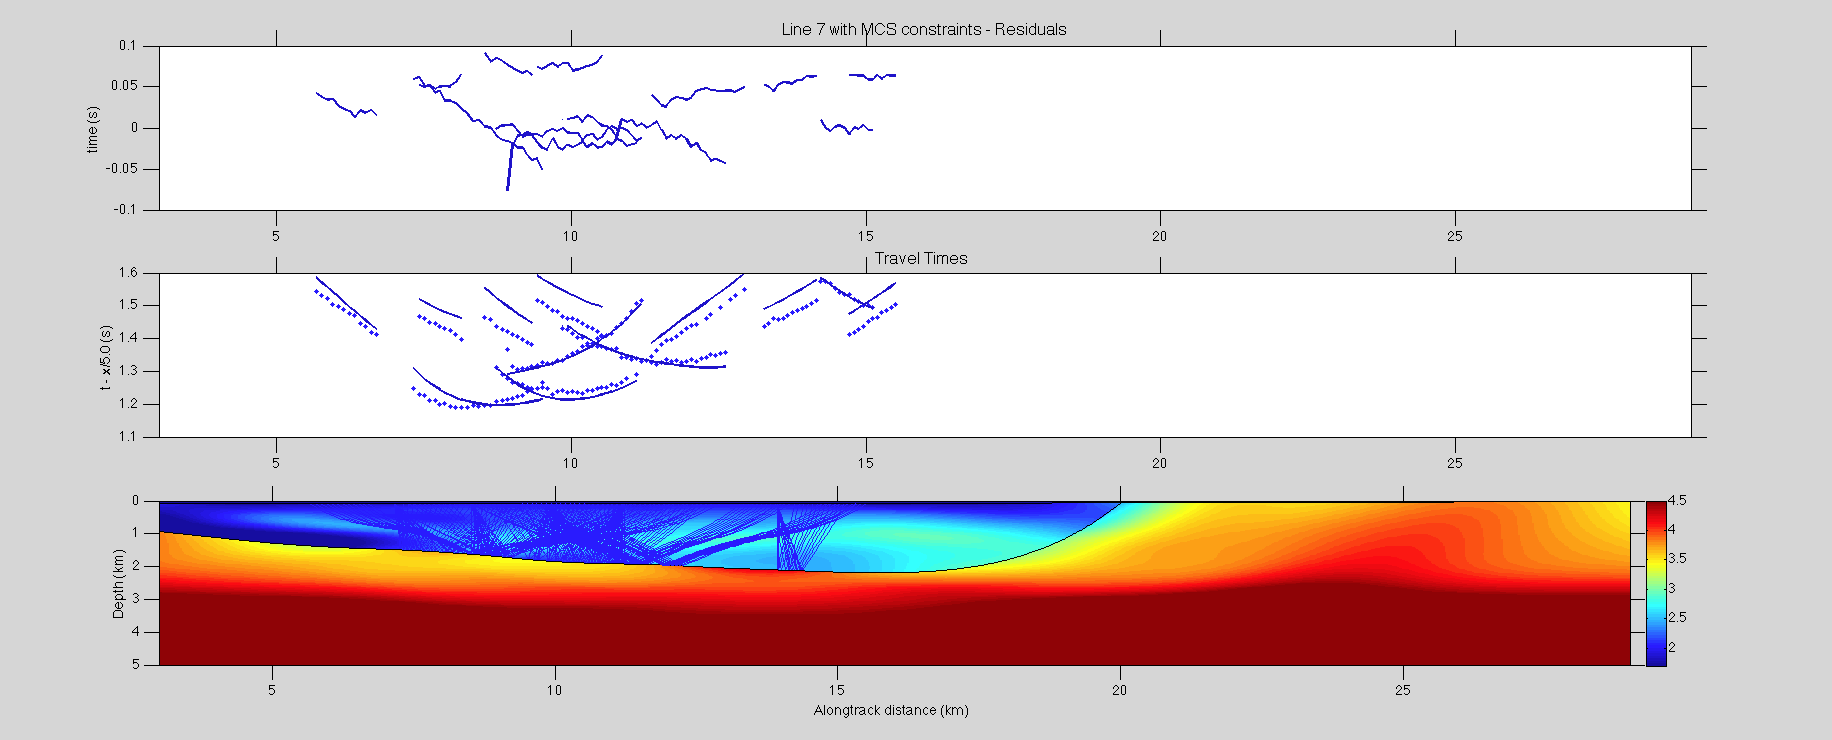
\includegraphics[scale=0.29,keepaspectratio=true]{figs/line7_resid_MCSconstraints.png}
\caption{Inversion 13 final model ray path residuals.}
\label{fig:line7MCS-resid}
\end{figure}


%Footnote example\footnote{Lorem ipsum dolor sit amet, consectetuer adipiscing elit.}.\\

%Citation example \cite{lamport94}.

%-----------------------------------------

\subexperiment{Inversion 14}

Start running inversions with varying interface surface traces.  For inversion 14, run an example with the SSAF trace set at x=18.94299186; this is commented in salton7base\_manip2.m.  

The starting model is under inversion14, and is named salton7base\_14\_0.vm, seen in \autoref{fig:startm14}.  This inversion will include constraints from MCS data; therefore, the file salton7base\_1\_4.ray will be included; this is the ray file for the MCS reflector picks.  The raytracing csh file is salton7base\_raytr14.csh and includes append = 1, so that the rays from the MCS file will be appended to the rayfan.  

The other settings are as follows:

set maxnode = 300,        
set cmax = 0.75,
set gdx = 1041,
set gdy = 1,
set gdz = 323

set stx = 10,
set sty = 0,
set stz = 9,
set ang = 0.5

set tstat = 0.0,
set xextension = 2.0,
set yextension = 2.0

Rayfan plotting is in script 
plot\_salton7\_raypaths\_14.m.

The inversion csh file is salton7base\_14.csh.  The parameters are as follows:

set sr = 10.0, set sz = 5.0

set slh =  0.02,
set jph =  0.005,
set rfh =  0.1,
set tstath = 0.04

set reg0 =    1.0, set reg1 =    1.0, set reg2 =   4.0

set asr = 5.0

set crf = 2, set cjp = 1

\begin{figure}[h!]
\raggedleft
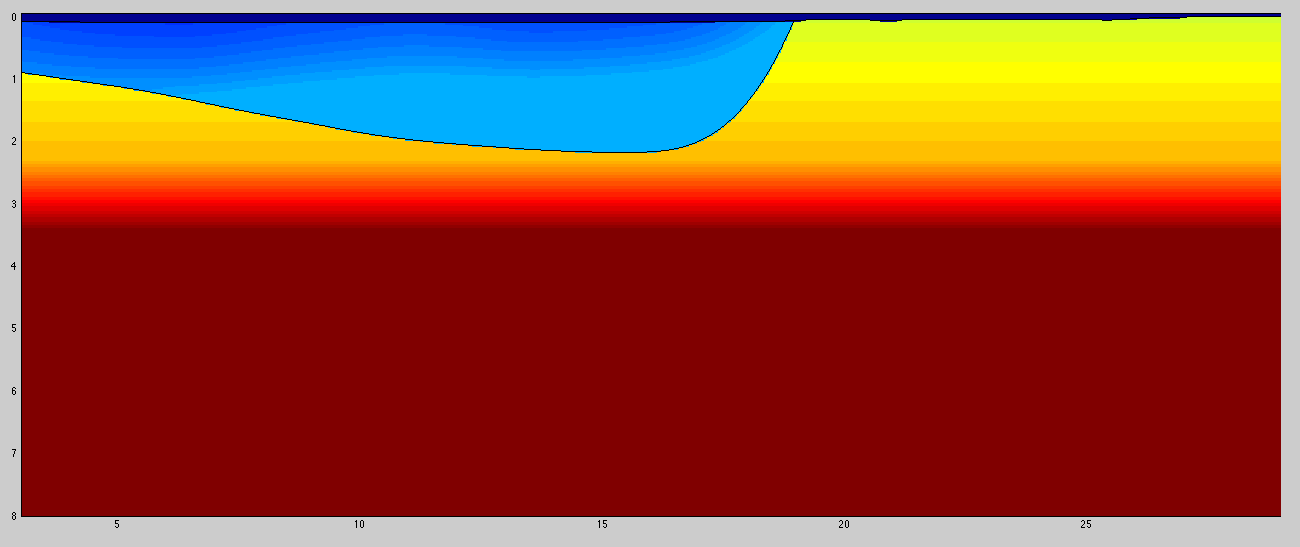
\includegraphics[scale=0.3,keepaspectratio=true]{figs/inv14_0.png}
\caption{Inversion 14 starting model.}
\label{fig:startm14}
\end{figure}







%-----------------------------------------

\subexperiment{Raytracing and Inversion Output}
Found in the tables \autoref{tab:r14}, \autoref{tab:i14}.
%\section{}
%Raytr it 
\begin{table}[ht]
\label{tab:r14}
\raggedleft
\begin{tabular}{c l l l l l}
\toprule
\textbf{Raytr, It = } & \textbf{tmean} & \textbf{trms} & \textbf{chi sq} & \textbf{chi r} & \textbf{meanErr} \\
\toprule
It0 & -0.0514 & 0.1174 & 73.2913 & 50.0788 & 0.0241\\
It1 & -0.0182 & 0.1075 & 47.3309 & 43.8783 & 0.0241\\
It2 & -0.0068 & 0.0906 & 25.6917 & 25.2468 & 0.0241\\
It3 & -0.0131 & 0.0644 & 14.3934 & 13.6786 & 0.0241\\
It4 & -0.0135 &  0.0527 & 8.7668 & 8.3057 & 0.0241\\
It5 & -0.0110 & 0.0446 & 5.2944 & 5.2898 & 0.0241\\
It6 & -0.0117 & 0.0382 & 3.1804 & 3.3014 & 0.0241\\
It7 & -0.0116 & 0.0360 & 2.5369 & 2.7169 & 0.0241\\
It8 & -0.0112 & 0.0349 & 2.2200 & 2.4544 & 0.0241\\
It9 & -0.0116 & 0.0339 & 2.0821 & 2.3345 & 0.0241\\
It10 & -0.0110 & 0.0338 & 1.9729 & 2.2349 & 0.0241\\
It11 & -0.0104 & 0.0336 & 1.9733 & 2.2920 & 0.0241\\
It12orig & -0.0108 & 0.0336 & 1.9329 & 2.2353 & 0.0241\\
It12 & -0.0039 & 0.0439 & 3.2228 & 3.4501 & 0.0241\\
It13 & -0.0114 & 0.0346 & 1.9718 & 2.1610 & 0.0241\\
It14 & -0.0112 & 0.0335 & 1.8335 & 2.1037 & 0.0241\\
It15 & -0.0101 & 0.0337 & 1.8931 & 2.2218 & 0.0241\\
It16 & -0.0120 & 0.0340 & 2.0673 & 2.2598 &  0.0241\\
\bottomrule\\
\end{tabular}
\caption{Inversion 14: Raytracing outputs.}
\end{table}

\clearpage

%INv it 
\begin{table}[ht]
\label{tab:i14}
\raggedleft
\begin{tabular}{c l l l}
\toprule
\textbf{Inv, It = } & \textbf{set chi sq =} & \textbf{out chi sq =} & \textbf{Penalty} \\
\toprule
It0 & 45 & 45.460 & 55886.17\\
It1 & 25 & 25.561 & 62766.52\\
It2 & 14 & 14.326 & 69724.12\\
It3 & 8 & 7.9459 & 75484.60\\
It4 & 5 & 4.9981 & 77469.94\\
It5 & 3 & 2.9994 & 86143.92\\
It6 & 2.3 & 2.3256 & 84903.17\\
It7 & 2.1 & 2.1429 & 81591.07\\
It8 & 1.8 & 1.8184 & 86594.72\\
It9 & 1.8 & 1.8618 & 83126.27\\
It10 & 1.8 & 1.8382 & 81169.54\\
It11 & 1.8 & 1.8382 & 79752.90\\
It12 & 2.0 & 2.0432 & 79529.48\\
It13 & 1.7 & 1.7128 & 83947.84\\
It14 & 1.7 & 1.7564 & 81046.24\\
It15 & 1.7 & 1.7376 & 79148.52\\
\bottomrule\\
\end{tabular}
\caption{Inversion 14: Inversion outputs.}
\end{table}

\clearpage

%----------------------------------------------------------------------------------------

\labday{Friday, 9 January 2015}
\experiment{Continuing Inversion 14}
Continuing from Thursday.  

\subexperiment{Inversion 14 steps and results}
Continued running Inversion 14 (output referenced in \autoref{tab:r14} and \autoref{tab:i14}).

Run nullspace shuttles on inversion iteration 11 (vm 12).  The pre-shuttled model, with a chi sq of 1.9329, is the best fit so far but is quite splotchy.  See in \autoref{fig:it11preshut}.  I used salton7\_shuttle\_update.m to create the shuttled model; 

\begin{figure}[h!]
\raggedleft
\includegraphics[scale=0.4,keepaspectratio=true]{../inversion14/figures/vm12_preshuttle.png}
\caption{Inversion 14, iteration 11 (vm 12), pre shuttle.}
\label{fig:it11preshut}
\end{figure}

Moving forwards, I named the output, shuttled model 

"Shuttles/line7shuttles/salton\_smshuttle\_inv14.vm".  This was copied into inversion14/, and renamed to salton7base\_14\_12.vm.
In inversion14, I renamed 12.ray, 12.vm, 12\_rough.vm, and 12\_raytr.out to orig.

In inversion\_temp, I renamed all iteration 11's to \_orig; including the anz, inz, nlr, rhsc, rhsn, sol, vecm\_in, and vecm\_out iteration 11's.  

\begin{figure}[h!]
\raggedleft
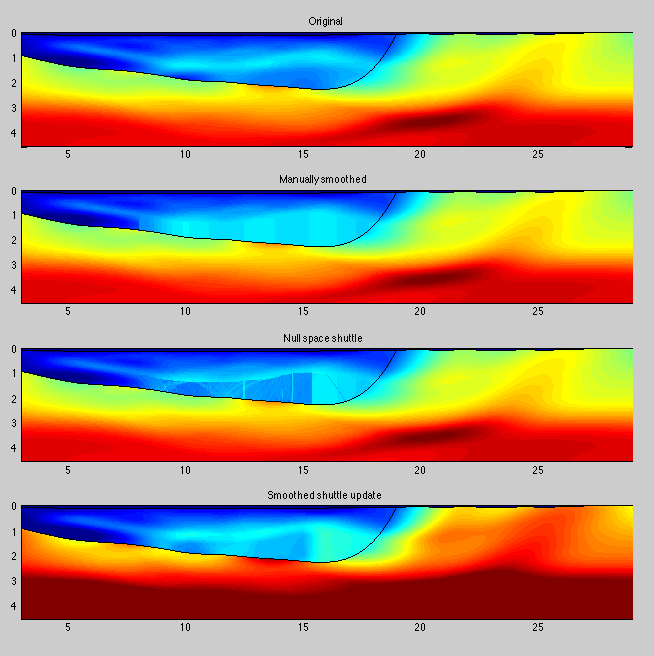
\includegraphics[scale=0.6,keepaspectratio=true]{figs/shuttlesInv14.png}
\caption{Inversion 14, iteration 11(vm12), post shuttle.}
\label{fig:it11postshut}
\end{figure}

After this, ray trace on the new shuttled model; so re-run raytracing iteration 12.  In the tables, the pre-shuttled statistics (raytracing it12) have been renamed to original.  The post-shuttled raytracing will be the new It12; this velocity model is in \autoref{fig:it11postshut}.

After several more iterations, I find that vm 14 (raytracing iteration 14, inversion iteration 13) has the lowest misfit (chi sq = 1.8335), and looks the "best" (the smoothest).  The final model is seen in \autoref{fig:inv14final}.  


\begin{figure}[h!]
\raggedleft
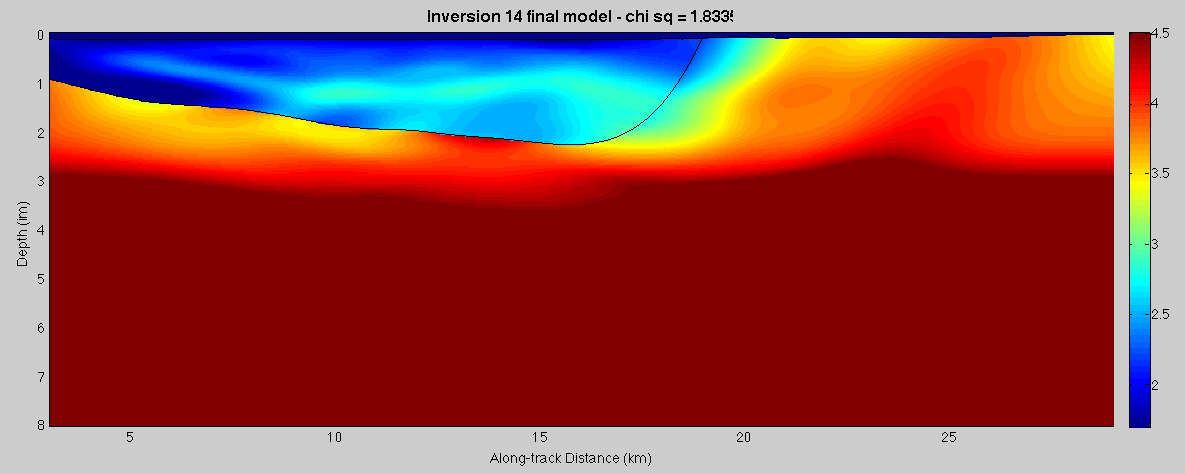
\includegraphics[scale=0.4,keepaspectratio=true]{figs/inv14_it13_FINAL.png}
\caption{Inversion 14, final model.  Vm number 14; chi sq = 1.8335.}
\label{fig:inv14final}
\end{figure}

\clearpage{}

%\experiment{example}
%
%\begin{equation}
%\label{eq:emc}
%e = mc^2
%\end{equation}
%
%Example equation citation: \autoref{eq:emc}.


%----------------------------------------------------------------------------------------
\labday{Thursday, 15 January 2015}

\experiment{Inversion 15 - Interface to the W of the SSAF trace}

Starting inversion 15.  Here, the interface intersects the surface at 17.9km along-profile, about 1 km west of the surface trace of the SSAF.  

To create the starting model, I once again used the script salton7base\_manip2.m.    The output model (starting model) is salton7base\_15\_0.vm, in inversion15/.  This is seen in \autoref{fig:inv15start}.  This inversion will include constraints from MCS data; therefore, the file salton7base\_1\_4.ray will be included; this is the ray file for the MCS reflector picks.  The raytracing csh file is salton7base\_raytr15.csh and includes append = 1, so that the rays from the MCS file will be appended to the rayfan.  

The other settings are as follows:

set maxnode = 300,        
set cmax = 0.75,
set gdx = 1041,
set gdy = 1,
set gdz = 323

set stx = 10,
set sty = 0,
set stz = 9,
set ang = 0.5

set tstat = 0.0,
set xextension = 2.0,
set yextension = 2.0


Rayfan plotting is in script 
plot\_salton7\_raypaths\_15.m.

The inversion csh file is salton7base\_15.csh.  The parameters are as follows:

set sr = 10.0, set sz = 5.0

set slh =  0.02,
set jph =  0.005,
set rfh =  0.1,
set tstath = 0.04

set reg0 =    1.0, set reg1 =    1.0, set reg2 =   4.0

set asr = 5.0

set crf = 2, set cjp = 1

\begin{figure}[h!]
\raggedleft
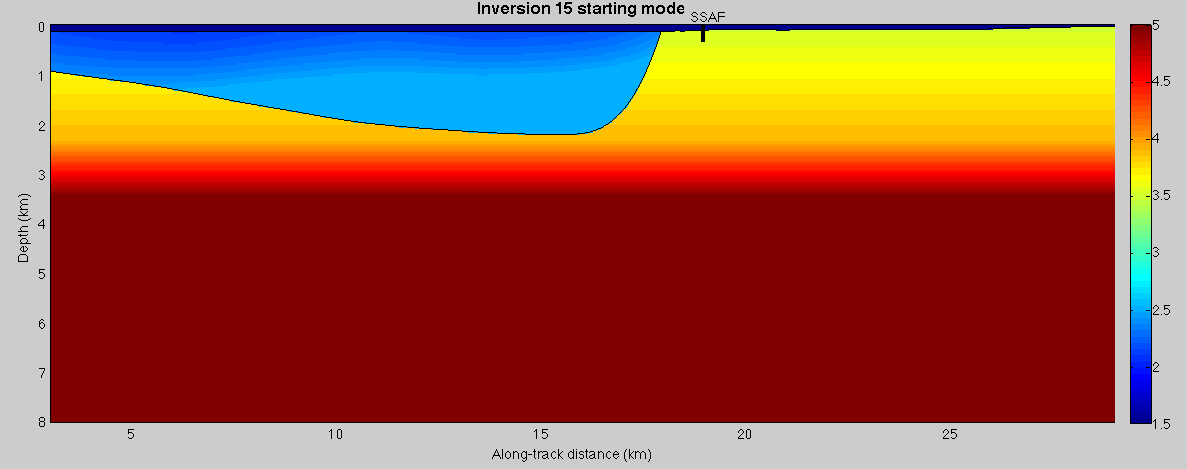
\includegraphics[scale=0.4,keepaspectratio=true]{figs/inv15_0.png}
\caption{Inversion 15 starting model.}
\label{fig:inv15start}
\end{figure}

\clearpage{}

\subexperiment{Raytracing and Inversion Output}
Output found in \autoref{tab:r15} and \autoref{tab:i15}.

%Raytracing Output, INversion 15
\begin{table}[!ht]
\label{tab:r15}
\raggedleft
\begin{tabular}{c l l l l l}
\toprule
\textbf{Raytr, It = } & \textbf{tmean} & \textbf{trms} & \textbf{chi sq} & \textbf{chi r} & \textbf{meanErr} \\
\toprule
It0 & -0.0529 & 0.1197 & 77.0745 & 52.4152 & 0.0241\\
It1 & -0.0222 & 0.1102 & 52.0758 & 47.1082 & 0.0241\\
It2 & -0.0055 & 0.0948 & 29.0273 & 28.6880 & 0.0241\\
It3 & -0.0134 & 0.0696 & 17.7654 & 16.8745 & 0.0241\\
It4 & -0.0135 & 0.0586 & 11.9874 & 11.4367 & 0.0241\\
It5 & -0.0111 & 0.0494 & 7.6122 & 7.5095 & 0.0241\\
It6 & -0.0098 & 0.0456 & 5.6006 & 5.6730 & 0.0241\\
It7 & -0.0105 & 0.0420 & 4.3647 & 4.4582 & 0.0241\\
It8 & -0.0110 & 0.0370 & 2.9838 & 3.1563 & 0.0241\\
It9 & -0.0112 & 0.0365 & 2.7190 & 2.9174 & 0.0241\\
It10 & -0.0109 & 0.0352 & 2.3849 & 2.6462 & 0.0241\\
It11 & -0.0104 & 0.0349 & 2.2980 & 2.5895 & 0.0241\\
It12 & -0.0113 & 0.0344 & 2.2386 & 2.4955 & 0.0241\\
It13 & -0.0107 & 0.0341 & 2.1513 & 2.4475 & 0.0241\\
\bottomrule\\
\end{tabular}
\caption{Inversion 15: Raytracing outputs.}
\end{table}

%Inversion Output, Inversion 15
%INv it 
\begin{table}[!ht]
\label{tab:i15}
\raggedleft
\begin{tabular}{c l l l}
\toprule
\textbf{Inv, It = } & \textbf{set chi sq =} & \textbf{out chi sq =} & \textbf{Penalty} \\
\toprule
It0 & 50 & 50.182 & 144875.5\\
It1 & 30 & 29.006 & 149535.8\\
It2 & 17 & 17.770 & 152034.2\\
It3 & 11 & 11.190 & 153989.8\\
It4 & 7 & 7.1052 & 159624.0\\
It5 & 5 & 5.2451 & 154047.7\\
It6 & 4 & 4.0112 & 153415.7\\
It7 & 3 & 2.8625 & 163787.0\\
It8 & 2.5 & 2.4805 & 158431.1\\
It9 & 2.3 & 2.3184 & 157304.5\\
It10 & 2.1 & 2.1941 & 155617.3\\
It11 & 2.0 & 2.0898 & 155357.0\\
It12 & 2.0 & 2.0662 & 153650.9\\
\bottomrule\\
\end{tabular}
\caption{Inversion 15: Inversion outputs.}
\end{table}

\subexperiment{Inversion 15 Results}
I did not run the nullspace shuttles method on this model.  It appears that the the misfit increases as the interface is moved further west; likewise, there are more artifacts observed in the model.  For previous inversions, the model fit the data with a lower misfit at the same place in the inversion.  The final model here has a chi sq of 2.1513, and can be seen in \autoref{fig:inv15final}.

\begin{figure}[h!]
\raggedleft
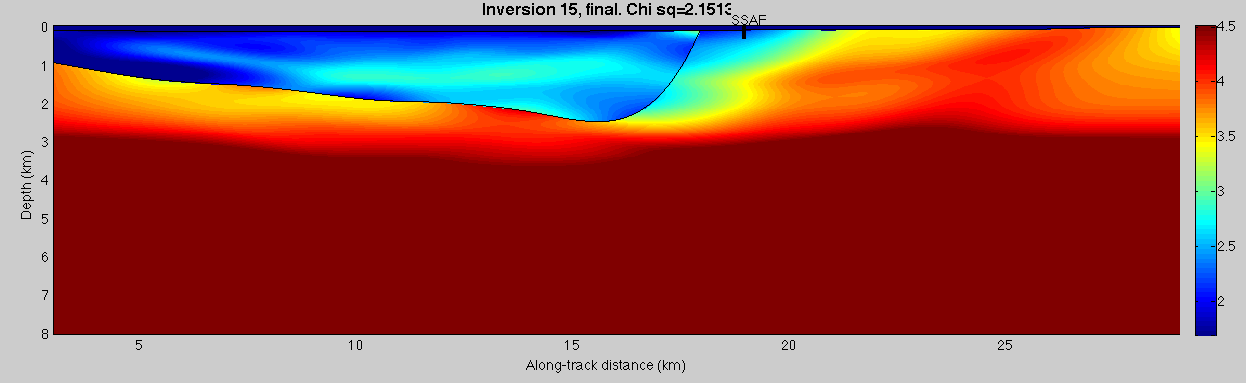
\includegraphics[scale=0.35,keepaspectratio=true]{figs/Inv15_final.png}
\caption{Inversion 15 final model, chi sq = 2.1513.}
\label{fig:inv15final}
\end{figure}


%-------------------------
%Inversion 16
\experiment{Inversion 16}
Here, I move the interface even further west of the SSAF.

\subexperiment{Inversion 16 setup}
In inversion 16, the interface intersects the surface at 15.9 km along-track distance.  The MCS data ends at approximately 15.5 km along-track distance, and I am including constraints from the MCS reflector times; therefore, I leave the bottom of the interface at 15.5 km depth where it is observed (and picked) in the constraining MCS data.  

To create the starting model, I used the same script as I did for the previous inversion (salton7base\_manip2.m).  The starting model can be seen in \autoref{fig:inv16start}.  As before, raytracing includes MCS reflector picks as a constraint for the interface, so append = 1 in the raytracing file.  The raytracing file has been copied from inversion 15 (and that from inversion 14), so all the parameters are the same as above.  Same for the inversion file.  The new raytracing and inversion files are, respectively, salton7base\_raytr16.csh and salton7base\_inv16.csh.  


\begin{figure}[h!]
\raggedleft
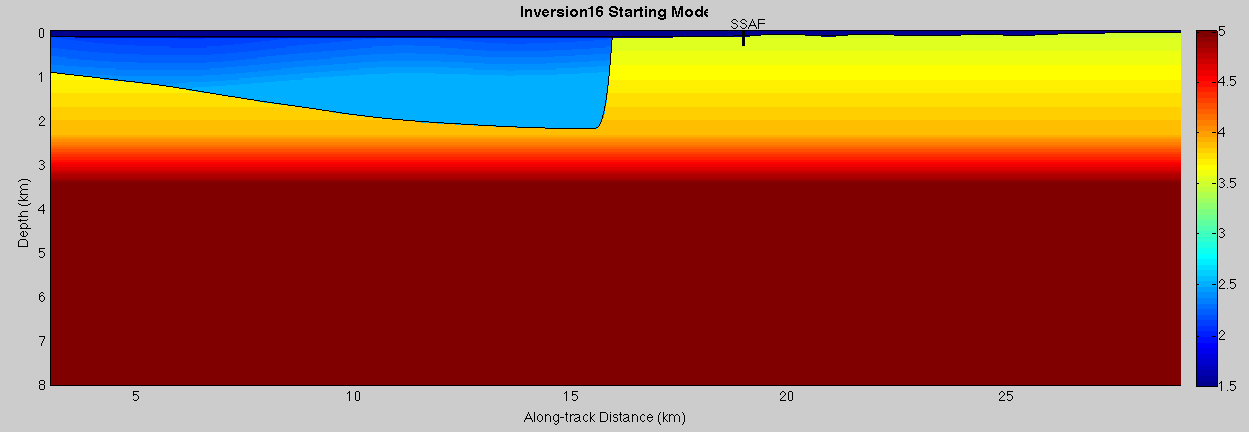
\includegraphics[scale=0.35,keepaspectratio=true]{figs/Inv16_0.png}
\caption{Inversion 16 starting model.}
\label{fig:inv16start}
\end{figure}

\subexperiment{Raytracing and Inversion Output}
Output found in \autoref{tab:r16} and \autoref{tab:i16}.

%Raytracing Output, I6version 16
\begin{table}[!ht]
\label{tab:r16}
\raggedleft
\begin{tabular}{c l l l l l}
\toprule
\textbf{Raytr, It = } & \textbf{tmean} & \textbf{trms} & \textbf{chi sq} & \textbf{chi r} & \textbf{meanErr} \\
\toprule
It0 & -0.0631 & 0.1416 & 112.2396 & 77.2975 & 0.0241\\
It1 & -0.0220 & 0.1136 & 54.0334 & 49.8177 & 0.0241\\
It2 & -0.0267 & 0.0811 & 28.8202 & 26.1150 & 0.0241\\
It3 & -0.0203 & 0.0724 & 26.8071 & 26.3205 & 0.0241\\
It4 & -0.0234 & 0.0688 & 20.0351 & 18.7892 & 0.0241\\
It5 & -0.0217 & 0.0666 & 18.0069 & 17.7185 & 0.0241\\
It6 & -0.0227 & 0.0591 & 12.1935 & 11.6280 & 0.0241\\
\bottomrule\\
\end{tabular}
\caption{Inversion 16: Raytracing outputs.}
\end{table}

%Inversion Output, Inversion 16
%Inv it 
\begin{table}[!ht]
\label{tab:i16}
\raggedleft
\begin{tabular}{c l l l}
\toprule
\textbf{Inv, It = } & \textbf{set chi sq =} & \textbf{out chi sq =} & \textbf{Penalty} \\
\toprule
It0 & 60 &  61.156 & 0.1114872E+08\\
It1 & 30 & 30.564 & 9220897\\
It2 & 20 & 20.267 & 8360667\\
It3 & 18 & 18.422 & 7846056\\
It4 & 15 & 15.474 & 7464322\\
It5 & 10 & 10.072 & 7227253\\
\bottomrule\\
\end{tabular}
\caption{Inversion 16: Inversion outputs.}
\end{table}

\subexperiment{Inversion 16 results}
It appears that this is too far west to place the interface-surface intersection; the interface dips too steeply.  After 5 iterations, I decided to stop running this; the misfit was not improving and the velocity model looks quite bad... \autoref{fig:inv16final}: 'nuff said. 

\begin{figure}[h!]
\raggedleft
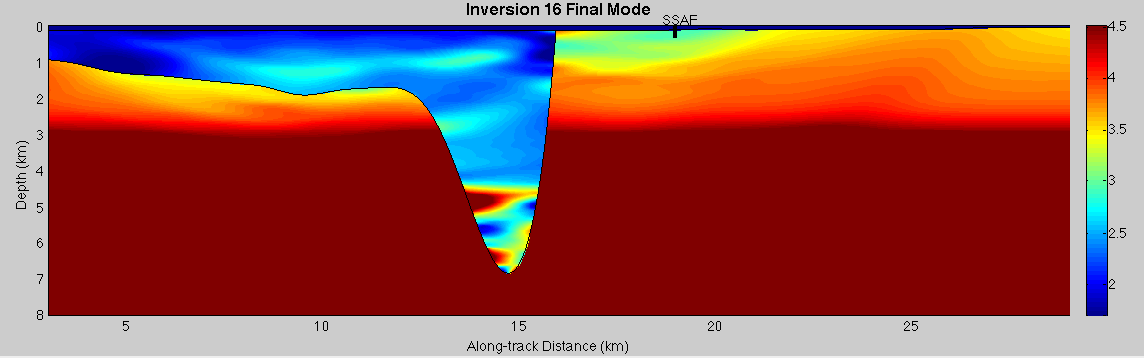
\includegraphics[scale=0.35,keepaspectratio=true]{figs/Inv16_final.png}
\caption{Inversion 16 final model.}
\label{fig:inv16final}
\end{figure}


%---------------------------------------------------------------------------------------------
\labday{Friday, 16 January 2015}
\experiment{Move Interface East of the SSAF Surface trace - Inversion 17}
The next few inversions are to explore the fit of an interface that intersects the surface to the east of the SSAF surface trace.  

\subexperiment{Inversion 17 Setup}
Inversion 12/13 had the interface at 20km along-track distance, which is approximate 1 km to the east of the SSAF surface trace.

Inversion 17 places the interface at 21.9 km along-track distance, which is ~ 3km to the east of the SSAF surface trace.  Again, salton7base\_manip2.m was used to create the starting model, which can be seen in \autoref{fig:inv17start}.  This was copied into the directory inversion17, from which this model will be run.

The parameters are the same as the past several inversions, and MCS reflector picks are included to constrain the interface depth.  

The raytracing file is salton7base\_raytr17.csh, and the inversion file is salton7base\_inv17.csh.  

\begin{figure}[h!]
\raggedleft
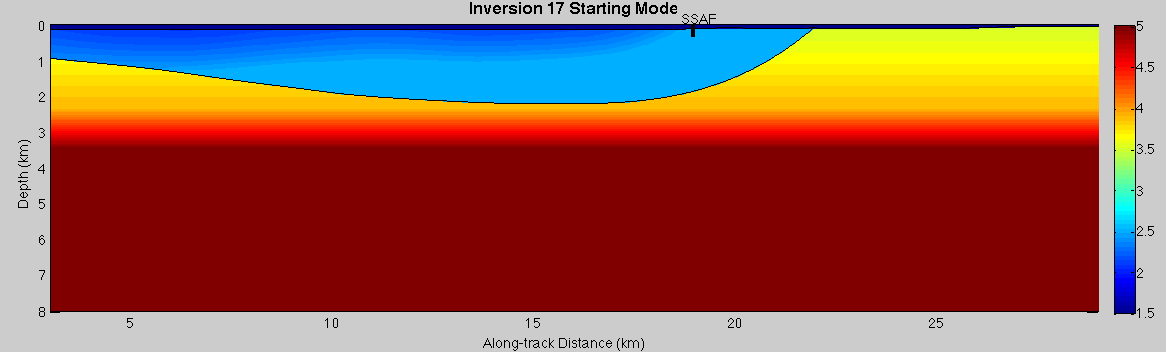
\includegraphics[scale=0.4,keepaspectratio=true]{figs/Inv17_0.png}
\caption{Inversion 17 starting model.}
\label{fig:inv17start}
\end{figure}

\subexperiment{Inversion 17 Raytracing and Inversion Output}

 %Raytracing Output, Inversion 17
\begin{table}[!ht]
\label{tab:r17}
\raggedleft
\begin{tabular}{c l l l l l}
\toprule
\textbf{Raytr, It = } & \textbf{tmean} & \textbf{trms} & \textbf{chi sq} & \textbf{chi r} & \textbf{meanErr} \\
\toprule
It0 & -0.0454 & 0.1084 & 59.1925 & 41.4194 & 0.0241\\
It1 & -0.0158 & 0.0990 & 37.0039 & 34.5539 & 0.0241\\
It2 & -0.0048 & 0.0853 & 20.1304 & 19.9383 & 0.0241\\
It3 & -0.0087 & 0.0745 & 15.2529 & 14.8563 & 0.0241\\
It4 & -0.0075 & 0.0624 & 10.0163 & 9.9648 & 0.0241\\
It5 & -0.0079 & 0.0553 & 7.3091 & 7.3324 & 0.0241\\
It6 & -0.0098 & 0.0467 & 5.0138 & 5.0799 & 0.0241\\
It7\_orig & -0.0097 & 0.0433 & 3.9889 & 4.1470 & 0.0241\\
It8\_orig & -0.0106 & 0.0391 & 3.1342 & 3.3032 & 0.0241\\
It9\_orig & -0.0115 & 0.0368 & 2.5874 & 2.7596 & 0.0241\\
It7 & -0.0056 & 0.0568 & 6.5518 & 6.6610 & 0.0241\\
It8 & -0.0124 & 0.0428 & 4.3133 & 4.2603 & 0.0241\\
It9 & -0.0109 & 0.0391 & 3.0443 & 3.2042 & 0.0241\\
It10 & -0.0111 & 0.0370 & 2.5758 & 2.7711 & 0.0241\\
It11 & -0.0118 & 0.0351 & 2.2134 & 2.4003 & 0.0241\\
It12 & -0.0111 & 0.0347 & 2.0743 & 2.3365 & 0.0241\\
It13 & -0.0112 & 0.0340 & 1.9712 & 2.2259 & 0.0241\\
It14 & -0.0107 & 0.0344 & 1.9761 & 2.2546 & 0.0241\\
It15 & -0.0109 & 0.0338 & 1.8934 & 2.1826 & 0.0241\\
It16 & -0.0108 & 0.0337 & 1.8875 & 2.1801 & 0.0241\\
\bottomrule\\
\end{tabular}
\caption{Inversion 17: Raytracing outputs.}
\end{table}

%Inversion Output, Inversion 17
%Inv it 
\begin{table}[!ht]
\label{tab:i17}
\raggedleft
\begin{tabular}{c l l l}
\toprule
\textbf{Inv, It = } & \textbf{set chi sq =} & \textbf{out chi sq =} & \textbf{Penalty} \\
\toprule
It0 & 35 &  35.220 & 13802.58\\
It1 & 20 & 19.960 & 18595.53\\
It2 & 15 & 15.165 & 14939.56\\
It3 & 10 & 9.9271 & 16998.00\\
It4 & 7 & 7.2088 & 19035.86\\
It5 & 5 & 5.0090 & 23574.42\\
It6 & 4 & 4.0140 & 24373.59\\
It7\_orig & 3 & 3.0159 & 29915.57\\
It8\_orig & 2.5 & 2.4266 & 35008.20\\
It7 & 4 & 4.0609 & 27968.18\\
It8 & 3 & 2.9973 & 33597.40\\
It9 & 2.5 & 2.4453 & 34715.13\\
It10 & 2.0 & 2.0206 & 41483.15\\
It11 & 1.9 & 1.9327 & 38489.62\\
It12 & 1.8 & 1.8218 & 39072.30\\
It13 & 1.8 & 1.8698 & 33794.29\\
It14 & 1.8 & 1.8090 & 33865.78\\
It15 & 1.8 & 1.7680 & 32857.09\\
\bottomrule\\
\end{tabular}
\caption{Inversion 17: Inversion outputs.}
\end{table}

\clearpage{}

\subexperiment{Inversion 17 Shuttles}
After Inversion iteration 6 (velocity model 7 and raytracing iteration 7), more artifacts become present in the model.  The chi sq of inversion iteration 6 is 3.9889; I run the nullspace shuttles method to update this model and rerun the inversions.  The pre-shuttle model is seen in \autoref{fig:inv17preshut}.

\begin{figure}[h!]
\raggedleft
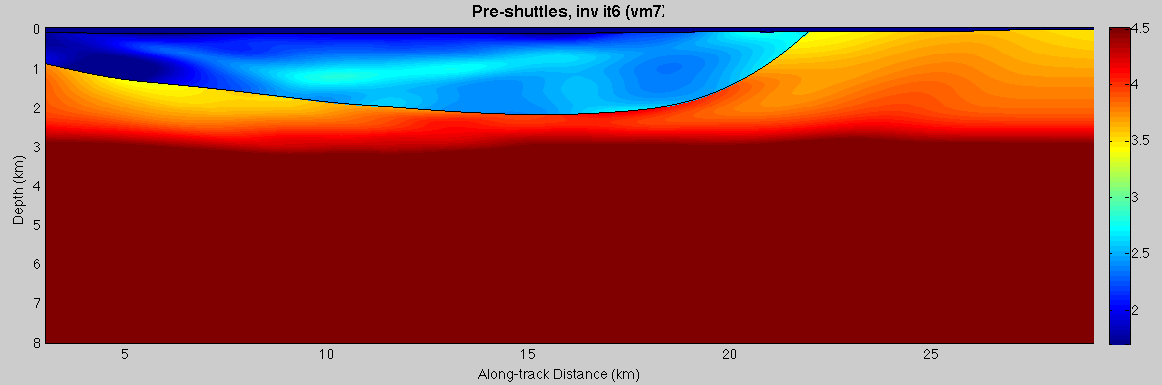
\includegraphics[scale=0.4,keepaspectratio=true]{figs/inv17preshut.png}
\caption{Inversion 17, pre-shuttles method.  Inversion iteration 6; chi sq = 3.9889.}
\label{fig:inv17preshut}
\end{figure}

There is a low velocity patch to east of the sedimentary basin; the main shuttles code (salton7\_shuttle\_update.m) maintains this low velocity patch and does not smooth it because of the current algorithm for updating ("filtering") the model.  This is seen in \autoref{fig:inv17postshut_o}.  

\begin{figure}[h!]
\raggedleft
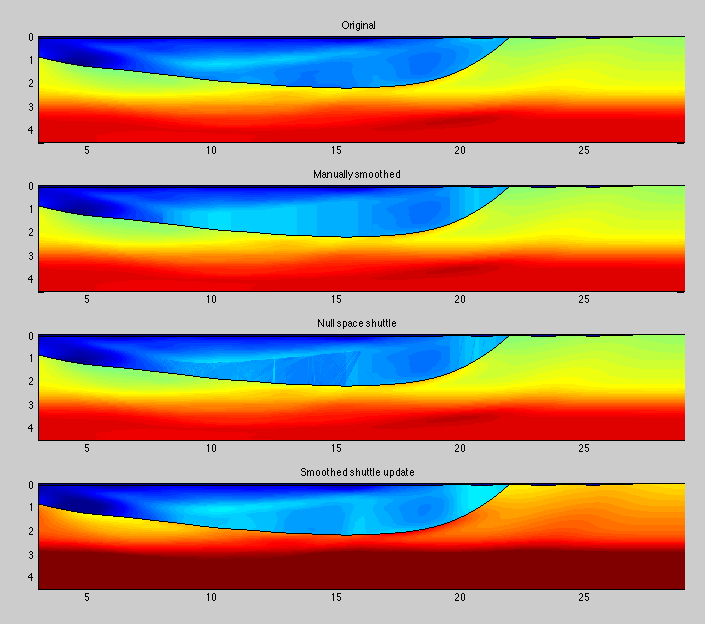
\includegraphics[scale=0.6,keepaspectratio=true]{figs/inv17postshut_orig.png}
\caption{Inversion 17, post-shuttles method with the original shuttles script.}
\label{fig:inv17postshut_o}
\end{figure}

To fix this, I added some conditionals in the filtering portion of the code; these changes are in salton7\_shuttle\_update\_in17.m.  I run this on inversion iteration 6 to get the newly shuttled model.  This shuttled model (and other info) can be seen in \autoref{fig:inv17postshut}.

\begin{figure}[h!]
\raggedleft
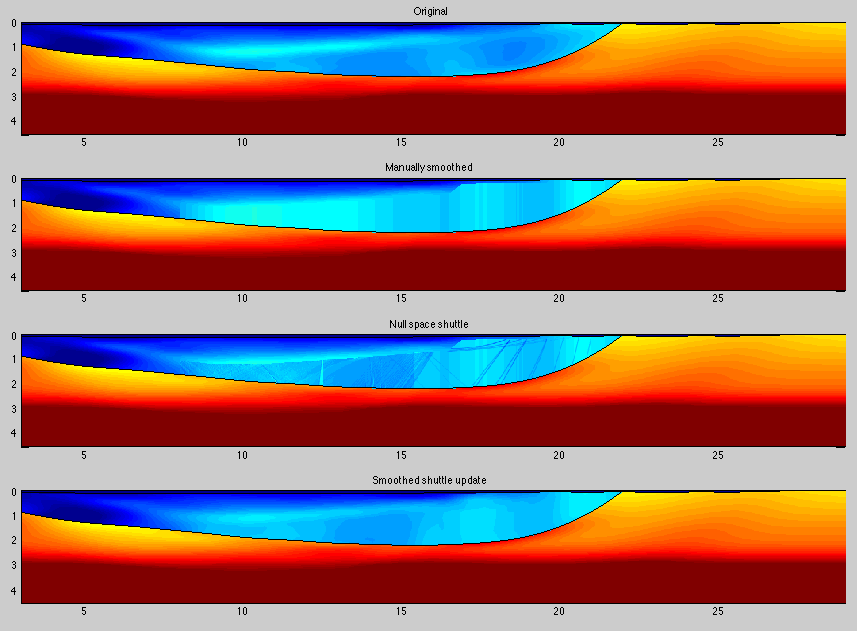
\includegraphics[scale=0.4,keepaspectratio=true]{figs/inv17postshut.png}
\caption{Inversion 17, nullspace shuttles model.}
\label{fig:inv17postshut}
\end{figure}

The resulting model is in salton\_smshuttle\_inv17.vm, in the Shuttles/line7shuttles.  I copy this intone /inversion17, and name it salton7base\_17\_7.vm.  This will be the new vm 7, so the next iteration will be raytracing iteration 7 and then inversion iteration 7.  

Rename all inversion 17, iteration 7, and 8 files in the inversion\_temp directory to 7\_orig and 8\_orig; rename all iteration 7 files (anz, inz, nlr, rhsc, rhsn, sol, and vecm) to \_orig17.
In the inversion17 directory, rename all iteration 7, 8, and 9 files to \_orig.

Restart now by raytracing on this model; raytracing iteration 7.  In the tables, the pre-shuttle iterations of these will be named \_orig (so raytracing iterations 7, 8 and 9 and inversion iterations 7 and 8).

\subexperiment{Inversion 17 Results}
After inversion iteration 11, the velocities around the interface/surface intersection become very high/low relative to the remainder of the layer.  Because of this, I pick iteration 11 (Velocity model 12) as the final model, with chi sq = 2.07.  This is seen in \autoref{fig:inv17fin}.  The ray paths and residuals for this model are in \autoref{fig:inv17ray}.


\begin{figure}[h!]
\raggedleft
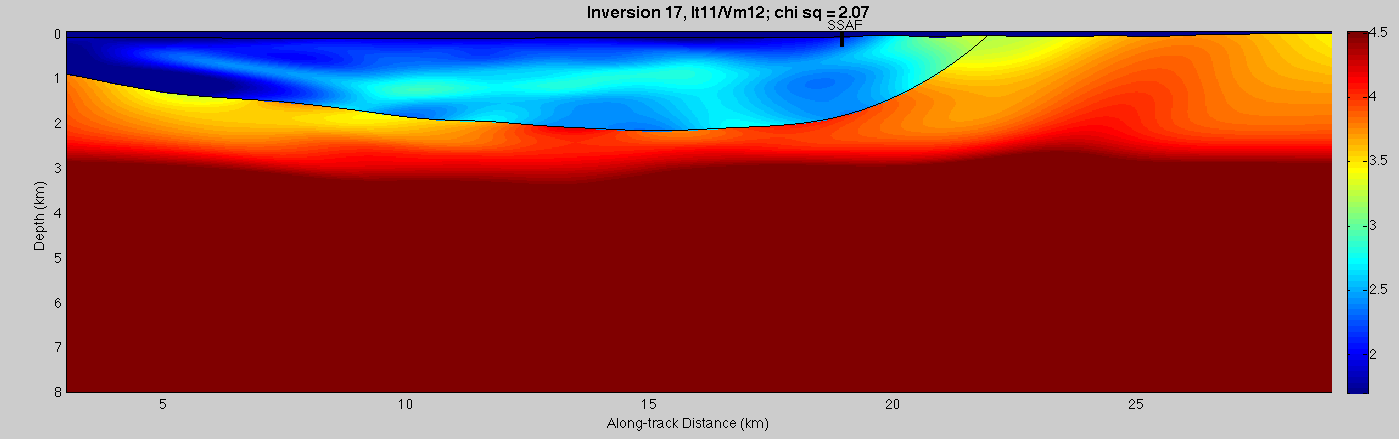
\includegraphics[scale=0.35,keepaspectratio=true]{figs/Inv17final.png}
\caption{Inversion 17, iteration 11 (vel model 12).  "Final" model, chi sq = 2.07.}
\label{fig:inv17fin}
\end{figure}

\begin{figure}[h!]
\raggedleft
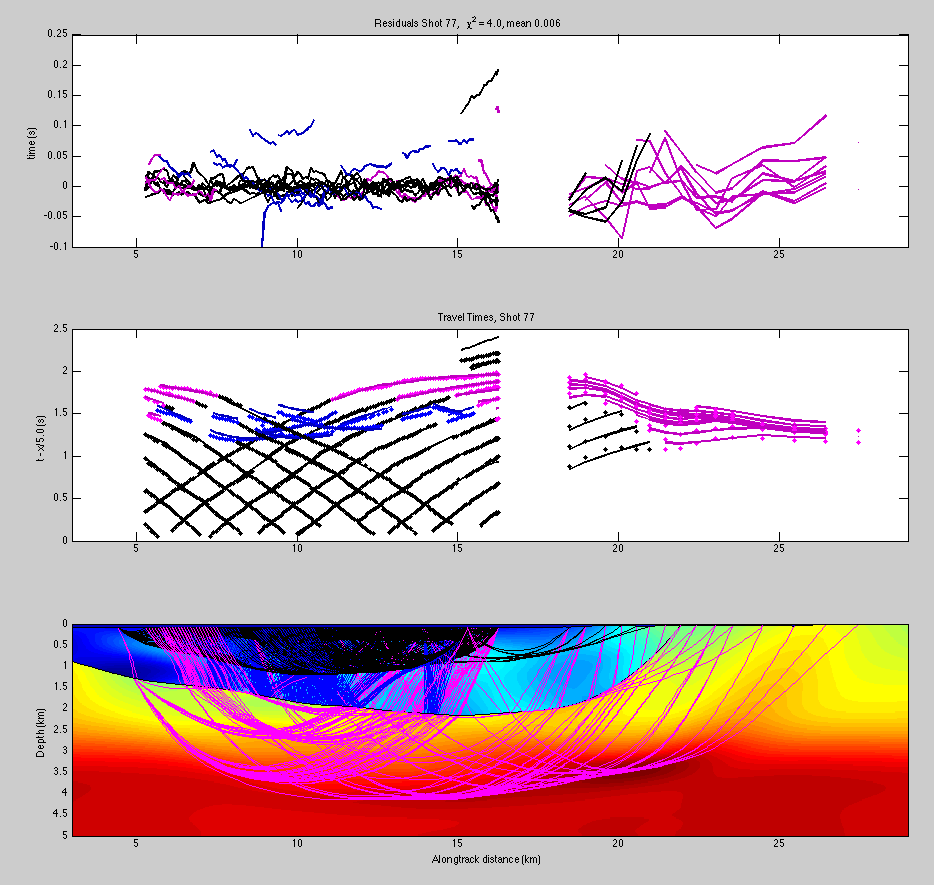
\includegraphics[scale=0.5,keepaspectratio=true]{figs/Inv17FinRay.png}
\caption{Inversion 17, final model, ray paths and residuals.}
\label{fig:inv17ray}
\end{figure}



\clearpage{}


%-------------Inversion 18-----------------
\experiment{Inversion 18}
Move the interface further west (5 km east of SSAF trace).

\subexperiment{Inversion 18 setup}
Here I move the interface surface intersection to 23.9 km along-track distance, which is ~5km to the east of the SSAF surface trace.  The script salton7base\_manip2.m is used to create the starting model salton7base\_18\_0.vm, seen in \autoref{fig:inv18start}, and in the directory inversion18.  

\begin{figure}[h!]
\raggedleft
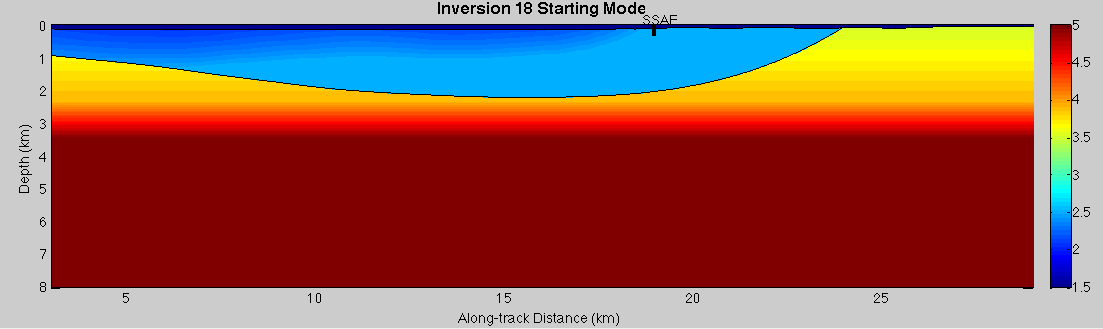
\includegraphics[scale=0.4,keepaspectratio=true]{figs/Inv18_0.png}
\caption{Inversion 18 starting model.}
\label{fig:inv18start}
\end{figure}

The scripts used are salton7base\_raytr18.csh and salton7base\_inv18.csh; the same parameters are used as the past several inversions, and MCS rays are used to constrain the interface (append = 1).  

\subexperiment{Inversion 18 Raytracing and Inversion Output}
See in tables 

 %Raytracing Output, Inversion 18
\begin{table}[!ht]
\label{tab:r18}
\raggedleft
\begin{tabular}{c l l l l l}
\toprule
\textbf{Raytr, It = } & \textbf{tmean} & \textbf{trms} & \textbf{chi sq} & \textbf{chi r} & \textbf{meanErr} \\
\toprule
It0 & -0.0415 & 0.1087 & 59.6053 & 44.9305 & 0.0241\\
It1 & -0.0185 & 0.1006 & 41.5355 & 38.4409 & 0.0241\\
It2 & -0.0066 & 0.0944 & 30.5015 & 30.0822 & 0.0241\\
It3 & -0.0077 & 0.0762 & 17.4766 & 17.2563 & 0.0241\\
It4 & -0.0096 & 0.0603 & 10.7631 & 10.6810 & 0.0241\\
It5 & -0.0110 & 0.0520 & 7.0319 & 6.9810 & 0.0241\\
It6 & -0.0110 & 0.0453 & 4.9075 & 5.0264 & 0.0241\\
It7\_orig & -0.0105 & 0.0428 & 4.0593 & 4.2240 & 0.0241\\
It7 & -0.0083 & 0.0546 & 6.4912 & 6.5738 & 0.0241\\
It8 & -0.0097 & 0.0474 & 5.1137 & 5.2320 & 0.0241\\
It9 & -0.0099 & 0.0431 & 3.9336 & 4.0762 & 0.0241\\
It10 & -0.0103 & 0.0393 & 3.0517 & 3.2352 & 0.0241\\
It11 & -0.0108 & 0.0371 & 2.5810 & 2.7943 & 0.0241\\
It12 & -0.0118 & 0.0351 & 2.2893 & 2.4825 & 0.0241\\
It13 & -0.0110 & 0.0345 & 2.0634 & 2.3417 & 0.0241\\
It14 & -0.0112 & 0.0341 & 2.0394 & 2.3096 & 0.0241\\
It15 & -0.0111 & 0.0338 & 1.9382 & 2.2083 & 0.0241\\
It16 & -0.0104 & 0.0338 & 1.9337 & 2.2528 & 0.0241\\
It17 & -0.0108 & 0.0337 & 1.9035 & 2.1977 & 0.0241\\
\bottomrule\\
\end{tabular}
\caption{Inversion 18: Raytracing outputs.}
\end{table}

%Inversion Output, Inversion 18
%Inv it 
\begin{table}[!ht]
\label{tab:i18}
\raggedleft
\begin{tabular}{c l l l}
\toprule
\textbf{Inv, It = } & \textbf{set chi sq =} & \textbf{out chi sq =} & \textbf{Penalty} \\
\toprule
It0 & 40 & 39.992 & 8932.743\\
It1 & 30 & 30.241 & 8148.220\\
It2 & 18 & 17.529 & 15017.25\\
It3 & 11 & 10.602 & 18093.48\\
It4 & 7 & 6.9742 & 19841.03\\
It5 & 5 & 4.9734 & 22544.40\\
It6 & 4 & 4.0191 & 21136.95\\
It7 & 5 & 5.0950 & 19466.58\\
It8 & 4 & 3.9825 & 19439.88\\
It9 & 3 & 3.5683 & 17018.32\\
It10 & 2.5 & 2.5128 & 27059.59\\
It11 & 2.0 & 2.0141 & 35238.67\\
It12 & 1.9 & 1.9400 & 35232.77\\
It13 & 1.8 & 1.8323 & 37072.04\\
It14 & 1.8 & 1.8397 & 35876.99\\
It15 & 1.8 & 1.8315 & 34804.32\\
It16 & 1.8 & 1.8277 & 33951.56\\
\bottomrule\\
\end{tabular}
\caption{Inversion 18: Inversion outputs.}
\end{table}

\clearpage{}

\subexperiment{Inversion 18 Shuttle Method}
Use the nullspace shuttles method on iteration 6 (velocity model and raytracing iteration 7); this model has a high velocity patch just at the surface (\autoref{fig:inv18preshut}).  

\begin{figure}[h!]
\raggedleft
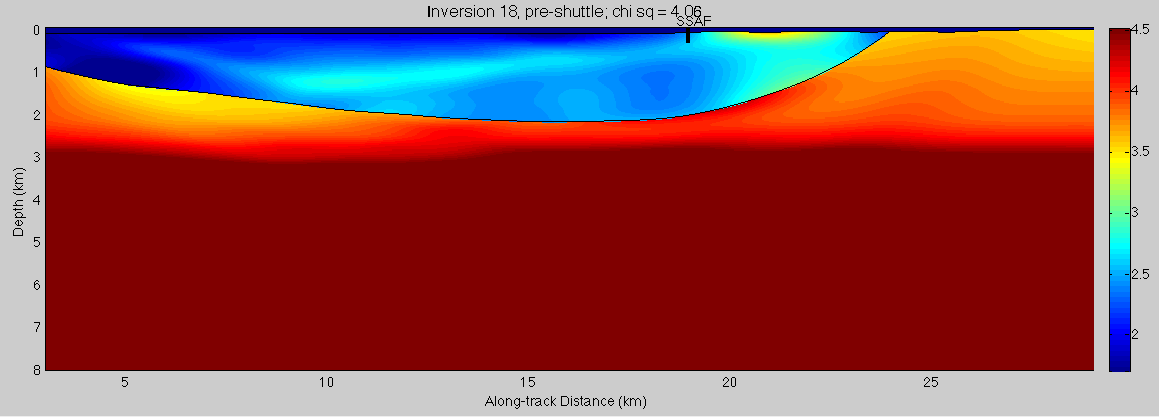
\includegraphics[scale=0.4,keepaspectratio=true]{figs/inv18_preshut.png}
\caption{Inversion 18, iteration 6, before using the shuttle method.  chi sq = 4.06.}
\label{fig:inv18preshut}
\end{figure}

Thus, the resulting shuttled velocity model have a streak of high velocity patch downwards into the model.  To create the shuttled model (the new velocity model 7), use the original shuttle script (salton7\_shuttle\_update.m).
Like all other shuttled inversions (except inversion 17), this takes the highest velocity observed in a  column in the first layer, and propagates it downwards to the basement interface.  The result in velocity model can be seen in \autoref{fig:inv18postshut}.

\begin{figure}[h!]
\raggedleft
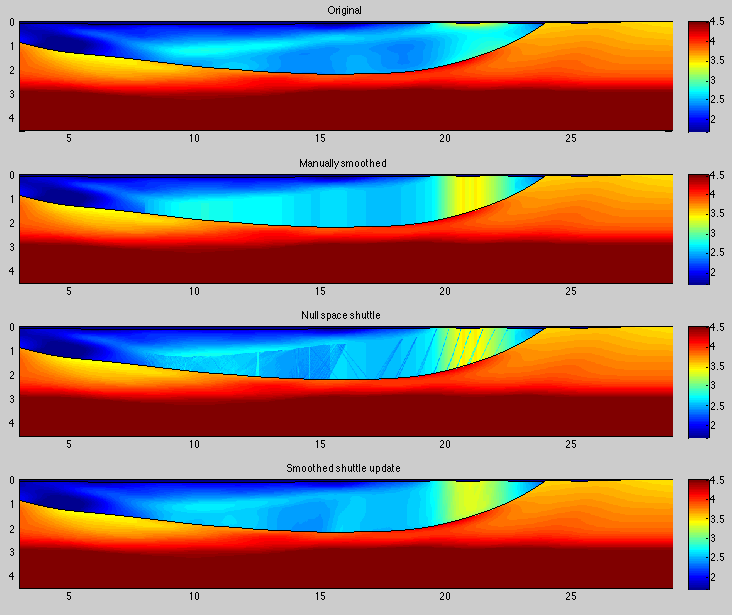
\includegraphics[scale=0.5,keepaspectratio=true]{figs/inv18_postshuttle.png}
\caption{Inversion 18, iteration 6, result of using the shuttles method on velocity model 7 (iteration 6).}
\label{fig:inv18postshut}
\end{figure} 
 
 This new velocity model is in the Shuttles/line7shuttles directory; it is salton\_smshuttle\_inv18.vm.  I copy this into inversion18 as salton7base\_18\_7.vm; the original velocity model 7 is renamed \_orig, as are raytracing iteration 7, rough.vm, raytracing output, and inversion iteration 6 output.  In the inversion\_temp directory, all inversion 18 iteration 6 jp, rf, and sl files are renamed to \_orig, as well as the iteration 6 anz, ins, nlr, rhsc, rhsn, sol, vecm\_in, and vem\_out.  
 
 In the raytracing output table, iteration 7 has been renamed to it7\_orig.  After copying the shuttled velocity model into the inversion17 directory, I re-raytrace through it in raytracing iteration 7.  This is the iteration 7 in the raytracing table.  
 
 After an iteration or two, it seems that the shuttles method should have been run on a model from a few iterations earlier, to avoid the large velocity patch; it seems to me that this may be unrealistic, and the inversion keeps re-updating so that the bottom is slower to accommodate the "pink" rays, as well as "black" rays.  I may run a separate inversion 19 in which i run nullspace shuttles earlier, to make the velocity more uniform and see what happens from here. 
 
 \subexperiment{Inversion 18 Results}
 After about iteration 14, the velocity model does not change much in appearance.  A low-velocity patch (~2.2 km/s) around 17 - 20 km develops, and a slightly higher velocity patch (3.1 - 3.6 km/s) in layer 1 develops around 21.2 km along-track distance.  However, the misfit improves over the course of the next 4 iterations, so I take the final iteration (inversion iteration 16, velocity model 17) to be the final model.  This can be seen in \autoref{fig:inv18final}.  
 
 
 \begin{figure}[h!]
\raggedleft
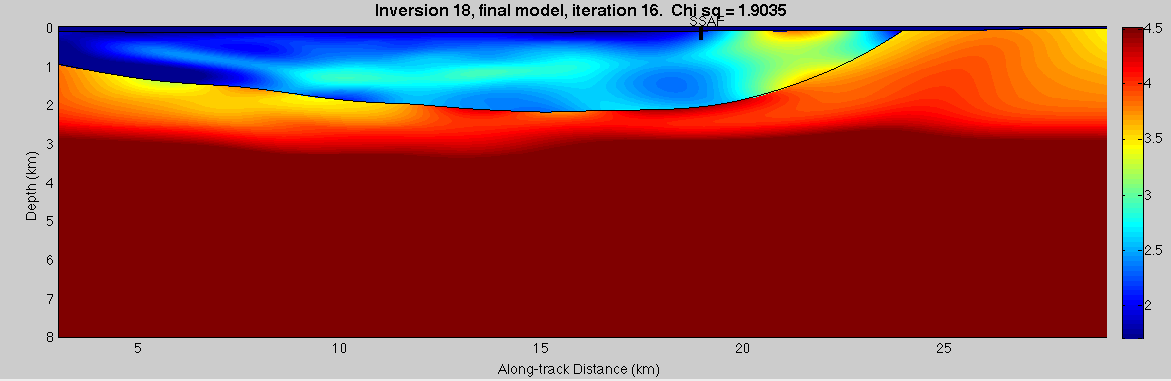
\includegraphics[scale=0.4,keepaspectratio=true]{figs/inv18final.png}
\caption{Inversion 18, inv iteration 16; velocity model 17.  Final model for inversion 18 with chi sq = 1.90.}
\label{fig:inv18final}
\end{figure} 
 
 The model with raypaths and residuals can be seen in \autoref{fig:inv18ray}

\begin{figure}[h!]
\raggedleft
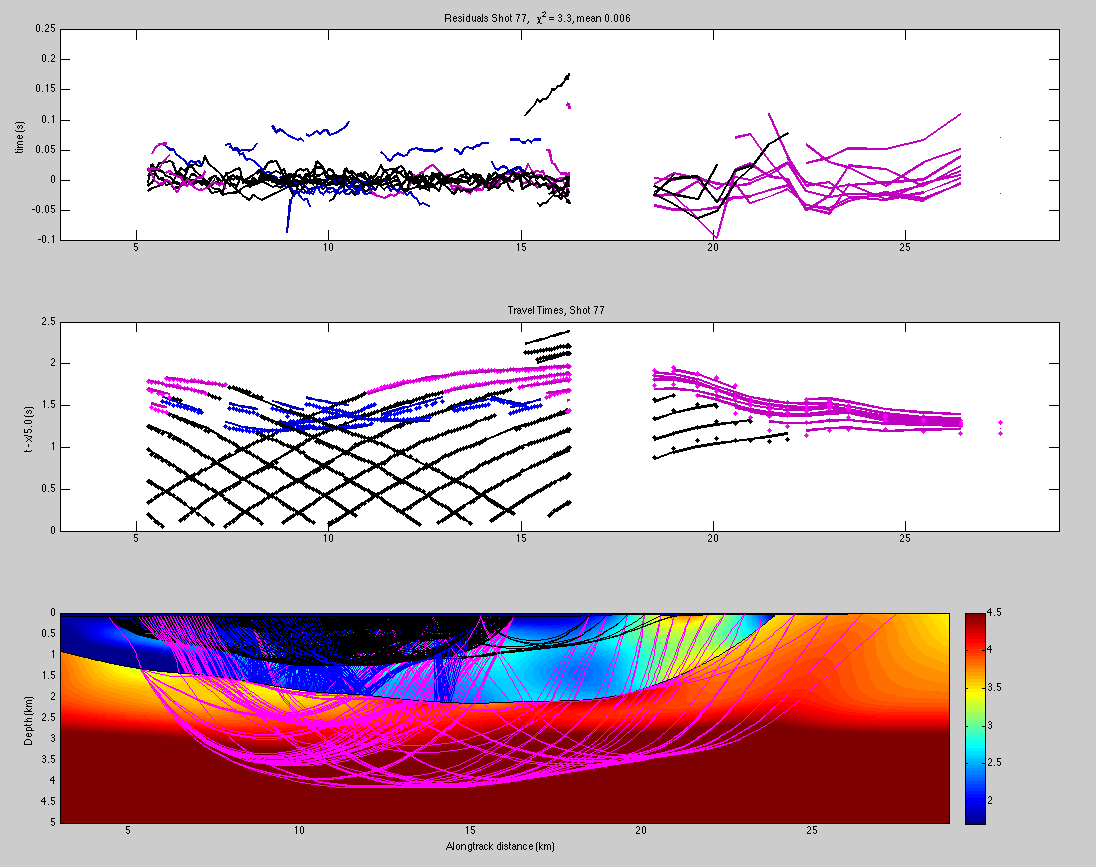
\includegraphics[scale=0.4,keepaspectratio=true]{figs/inv18finalRay.png}
\caption{Inversion 18, inv iteration 16; velocity model 17.  Raypaths and residuals.}
\label{fig:inv18ray}
\end{figure} 


%--------------------Inversion 19------------------------------------
\experiment{Inversion 19; Run shuttles earlier on inv 18}
I noticed on inversion 18 that the iteration on which I ran the shuttles may have influenced the end result of the high velocity patch in the east.  To test whether this is the case, I copy the first few iterations of inversion 18 into inversion 19 and run shuttles on an earlier iteration.  

\subexperiment{Inversion 19 Setup}
Run the nullspace shuttles method on inversion 18 iteration 5 (velocity model 6).  See \autoref{fig:inv19preshut} and \autoref{fig:inv19sshut}.  The resulting shuttled model is salton\_smshuttle\_inv19.vm, which I copy into the inversion 19 directory as salton7base\_19\_0.vm.  

\begin{figure}[h!]
\raggedleft
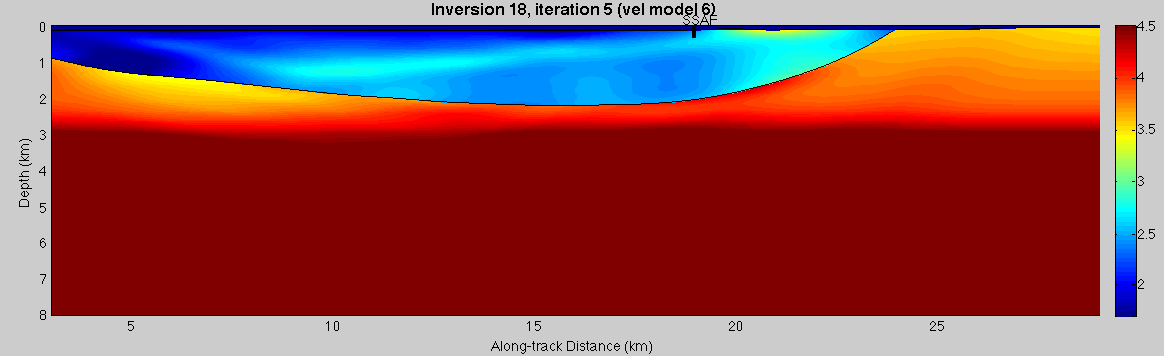
\includegraphics[scale=0.4,keepaspectratio=true]{figs/Inv18It5pre19.png}
\caption{Inversion 18, inv iteration 5 (velocity model 6).  chi sq = 4.91.  Run the shuttles method on this model to form the "starting" model for inversion 19.}
\label{fig:inv19preshut}
\end{figure} 

\begin{figure}[h!]
\raggedleft
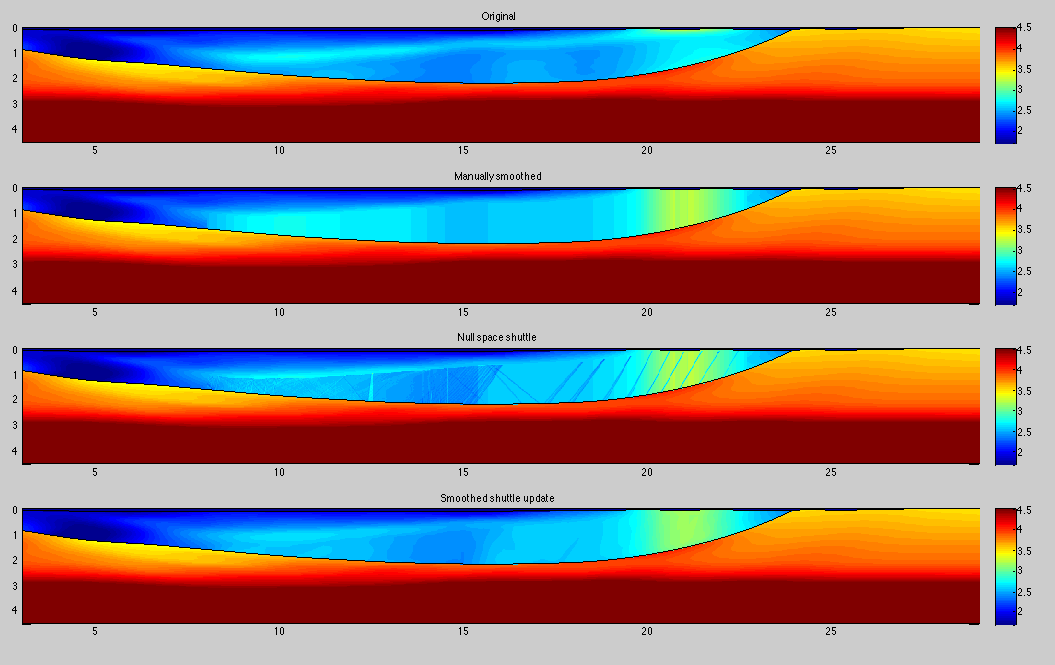
\includegraphics[scale=0.4,keepaspectratio=true]{figs/Inv19startshut.png}
\caption{Using the shuttles method on inversion 18 iteration 5; the bottom model will be the starting model for inversion 19.}
\label{fig:inv19sshut}
\end{figure} 

The starting model by itself can be seen in \autoref{fig:inv19start}.  I also copy over salton7base\_1\_4.ray.  

\begin{figure}[h!]
\raggedleft
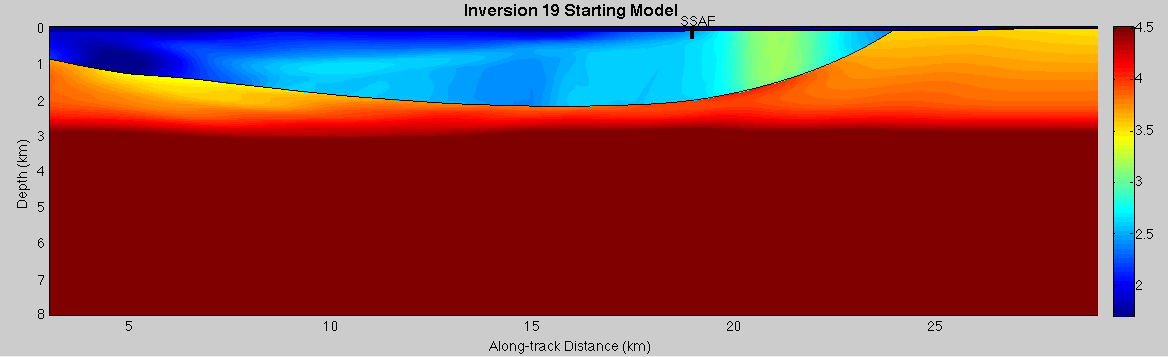
\includegraphics[scale=0.4,keepaspectratio=true]{figs/Inv19start.png}
\caption{Inversion 19 startin model.}
\label{fig:inv19start}
\end{figure} 

To run the inversion, I use the same parameters as before, in the files salton7base\_raytr19.csh and salton7base\_inv19.csh.

\clearpage{}

\subexperiment{Inversion 19 Raytracing and Inversion Output}
Raytracing and Inversion output can be seen in \autoref{tab:r19} and \autoref{tab:i19}.
At inversion iteration 4, I change reg1 (first derivative smoothing) and reg2 (second derivative smoothing).  Before, these were set to reg1 = 1; reg2 = 4.  At iteration 4, I change reg1 = 5 and reg2 = 20.  

 %Raytracing Output, Inversion 19
\begin{table}[!ht]
\label{tab:r19}
\raggedleft
\begin{tabular}{c l l l l l}
\toprule
\textbf{Raytr, It = } & \textbf{tmean} & \textbf{trms} & \textbf{chi sq} & \textbf{chi r} & \textbf{meanErr} \\
\toprule
It0 & -0.0080 & 0.0610 & 8.3738 & 8.3645 & 0.0241\\
It1 & -0.0118 & 0.0461 & 5.3498 & 5.3419 & 0.0241\\
It2 & -0.0106 & 0.0427 & 3.9472 & 4.0706 & 0.0241\\
It3 & -0.0106 & 0.0389 & 3.0678 & 3.2368 & 0.0241\\
It4 & -0.0116 & 0.0364 & 2.4807 & 2.6565 & 0.0241\\
It5 & -0.0115 & 0.0348 & 2.1705 & 2.4027 & 0.0241\\ 
It6 & -0.0116 & 0.0345 & 2.1458 & 2.3752 & 0.0241\\
It7 & -0.0107 & 0.0347 & 2.0637 & 2.3439 & 0.0241\\
It8 & -0.0108 & 0.0345 & 2.0462 & 2.3489 & 0.0241\\
\bottomrule\\
\end{tabular}
\caption{Inversion 19: Raytracing outputs.}
\end{table}

%Inversion Output, Inversion 19
%Inv it 
\begin{table}[!ht]
\label{tab:i19}
\raggedleft
\begin{tabular}{c l l l}
\toprule
\textbf{Inv, It = } & \textbf{set chi sq =} & \textbf{out chi sq =} & \textbf{Penalty} \\
\toprule
It0 & 5 & 5.1420 & 24736.99\\
It1 & 4 & 4.0636 & 23474.95\\
It2 & 3 & 3.0132 & 27237.83\\
It3 & 2.4 & 2.3808 & 33565.06\\
It4 & 2 & 2.0072 & 957605.2\\
It5 & 1.9 & 1.9232 & 928151.3\\
It6 & 1.9 & 1.9913 & 798585.9\\
It7 & 1.9 & 1.9715 & 772211.0\\
\bottomrule\\
\end{tabular}
\caption{Inversion 19: Inversion outputs.}
\end{table}

\clearpage{}

\subexperiment{Inversion 19 Results}
I choose inversion iteration 5 (velocity model 6) as the "final" model for inversion 19; after this iteration, the fit does not improve much but the model becomes "splotchier".  The misfit for this model is 2.1458, and is in \autoref{fig:inv19fin}.  The ray paths and residuals are in \autoref{fig:inv19fray}.  In the lake, from about 3 to 16/17 km along-track distance, the first layer exhibits what are likely lake sediments.  From ~16 to ~20 km along-track distance, there is a lower velocity patch of approximately 2.5 km/s, lower than most of these lake sediments, and beyond this the velocities increase until layer 2 is reached.  the ray coverage in this region of varying velocities is approximately the same (mostly land shots, some marine shots), so I think this may be real.  This low velocity patch could be a damage zone related to the SSAF and another (normal!) fault, and the higher velocities to the east reflect the lacustrine, but compacted, Borrego Formation.

\begin{figure}[h!]
\raggedleft
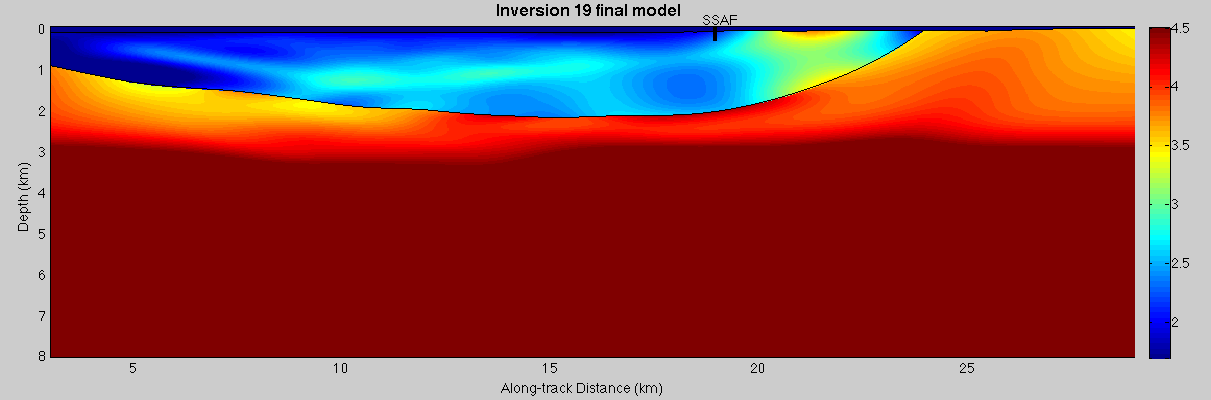
\includegraphics[scale=0.4,keepaspectratio=true]{figs/Inv19final.png}
\caption{Inversion 19 final model, chi sq = 2.1458.}
\label{fig:inv19fin}
\end{figure} 
 
\begin{figure}[h!]
\raggedleft
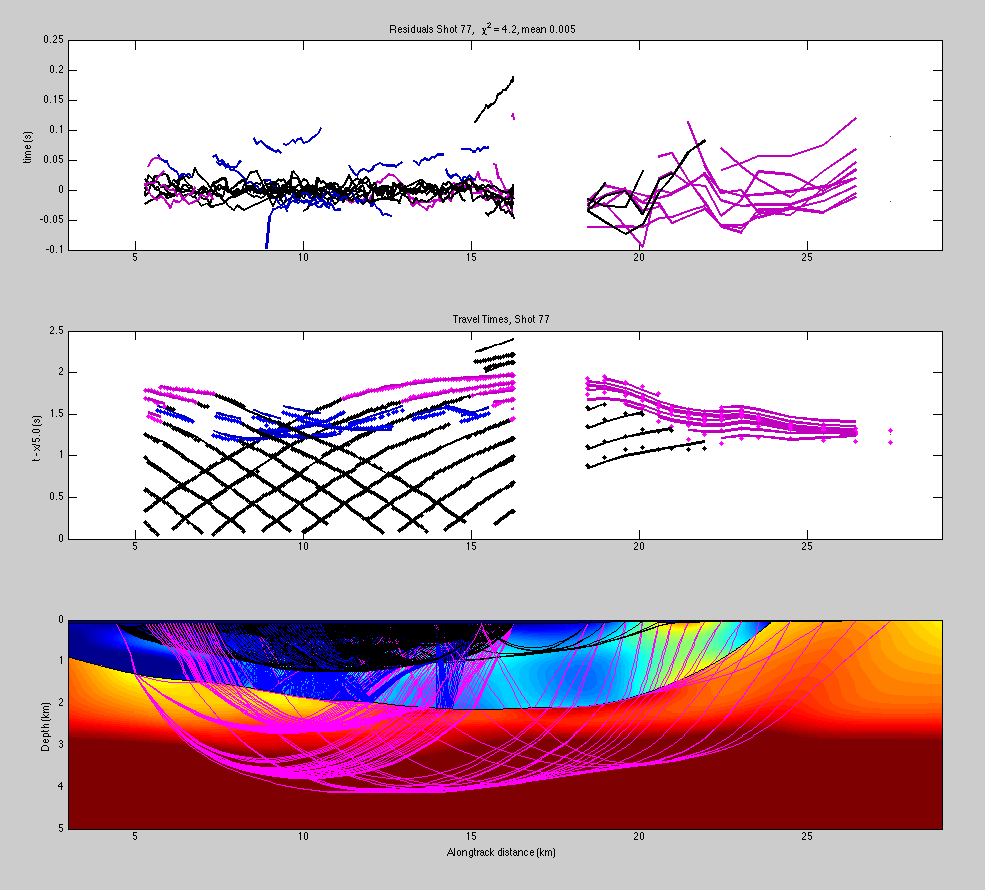
\includegraphics[scale=0.4,keepaspectratio=true]{figs/Inv19finalRay.png}
\caption{Inversion 19 final model, chi sq = 2.1458; ray paths and residuals.  The colorbar is the same as all the above figure (1.7 km/s to 4.5 km/s).}
\label{fig:inv19fray}
\end{figure} 
 
\clearpage{}

\experiment{Inversion 20: Inversion 17 without MCS constraints}
 Essentially running inversion 17 without including MCS constraints.
 
 \subexperiment{Inversion 20 setup}
Here I use the same starting model as inversion 17.  In this case, the interface intersects with the surface approximately 3 km to the east of the SSAF surface trace.  This model is created using salton7base\_manip2.m, and can be seen in \autoref{fig:inv17start}.   

I \textbf{do not} use constraints from interface picks in the MCS data; I wish to see how the velocity model develops without using these, so as to compare with inversion 17.  Therefore, in salton7base\_raytr20.csh, I set append = 0.  All the other parameters are the same as inversion 17.  Likewise, in salton7base\_inv20.csh, the parameters are all the same as inversion 17's inv shell script.

\subexperiment{Inversion 20 Raytracing and Inversion Output}
Seen in \autoref{tab:r20} and \autoref{tab:i20}.  

 %Raytracing Output, Inversion 20
\begin{table}[!ht]
\label{tab:r20}
\raggedleft
\begin{tabular}{c l l l l l}
\toprule
\textbf{Raytr, It = } & \textbf{tmean} & \textbf{trms} & \textbf{chi sq} & \textbf{chi r} & \textbf{meanErr} \\
\toprule
It0 & -0.0496 & 0.1317 & 91.4024 & 62.9833 & 0.0152\\
It1 & 0.0024 & 0.1184 & 53.2251 & 53.8442 & 0.0152\\
It2 & 0.0066 & 0.0990 & 30.3647 & 31.5226 & 0.0152\\
It3 & 0.0071 & 0.0828 & 20.7694 & 21.6819 & 0.0152\\
It4 & 0.0065 & 0.0688 & 14.2876 & 14.8850 & 0.0152\\
It5 & 0.0047 & 0.0558 & 9.2968 & 9.6312 & 0.0152\\
It6\_orig & 4.9578e-04 & 0.0444 & 6.2895 & 6.3200 & 0.0152\\
It7\_orig & -6.1330e-04 & 0.0357 & 4.2755 & 4.2476 & 0.0152\\
It6 & 0.0088 & 0.0660 & 10.9565 & 11.5418 & 0.0152\\
It7 & -1.1790e-04 & 0.0451 & 6.9680 & 6.9605 & 0.0152\\
It8 & 4.8140e-04 & 0.0415 & 5.2106 & 5.2368 & 0.0152\\
It9 & 3.7569e-04 & 0.0369 & 4.3638 & 4.3790 & 0.0152\\
It10 & -0.0015 & 0.0317 & 3.2893 & 3.2283 & 0.0152\\
It11 & -0.0020 & 0.0296 & 3.0128 & 2.9356 & 0.0152\\
It12 & -0.0027 & 0.0267 & 2.5557 & 2.4520 & 0.0152\\
It13 & -0.0017 & 0.0252 & 2.1650 & 2.1178 & 0.0152\\
It14 & -8.8259e-04 & 0.0250 & 2.0280 & 2.0115 & 0.0152\\
It15 & -9.5464e-04 &  0.0244 & 1.9192 & 1.9017 & 0.0152\\
It16 & -8.8819e-04 & 0.0241 & 1.8761 & 1.8646 & 0.0152\\
It17 & -0.0011 & 0.0247 & 1.9218 & 1.9047 & 0.0152\\
It18 & 6.8491e-05 & 0.0248 & 1.9649 & 1.9653 & 0.0152\\
It19 & -9.9049e-04 & 0.0245 & 1.9030 & 1.8900 & 0.0152\\
It20 & 1.9587e-05 & 0.0246 & 1.9414 & 1.9414 & 0.0152\\
\bottomrule\\
\end{tabular}
\caption{Inversion 20: Raytracing outputs.}
\end{table}

%Inversion Output, Inversion 20
%Inv it 
\begin{table}[!ht]
\label{tab:i20}
\raggedleft
\begin{tabular}{c l l l}
\toprule
\textbf{Inv, It = } & \textbf{set chi sq =} & \textbf{out chi sq =} & \textbf{Penalty} \\
\toprule
It0 & 50 & 51.104 & 14107.46\\
It1 & 30 & 29.685 & 17073.58\\
It2 & 20 & 20.422 & 17092.00\\
It3 & 14 & 14.005 & 17744.63\\
It4 & 9 & 8.9986 & 21881.66\\
It5 & 6 & 5.8927 & 25123.21\\
It6\_orig & 4 & 4.0016 & 30759.92\\
It6 & 6 & 6.1300 & 25204.87\\
It7 & 5 & 5.0299 & 23606.95\\
It8 & 4 & 4.0304 & 23084.88\\
It9 & 3 & 3.0037 & 28845.18\\
It10 & 2.5 & 2.4586 & 28798.93\\
It11 & 2.0 & 2.0127 & 33113.56\\
It12 & 1.8 & 1.8486 & 30816.13\\
It13 & 1.8 &1.8236 & 27384.25\\
It14 & 1.8 & 1.7716 & 25599.62\\
It15 & 1.8 & 1.7144 & 24697.77\\
It16 & 1.8 & 1.8243 & 21345.34\\
It17 & 1.8 & 1.9951 & 18642.92\\
It18 & 1.8 & 1.8336 & 19567.24\\
It19 & 1.8 & 1.8467 & 18806.85\\
\bottomrule\\
\end{tabular}
\caption{Inversion 20: Inversion outputs.}
\end{table}

\clearpage{}

\subexperiment{Inversion 20 shuttles}
I run the shuttle method on inversion iteration 5 (velocity model 6) of inversion 20.  Velocity model 6 can be seen in \autoref{fig:inv20preshut}.  I used the script salton7\_shuttle\_update\_inv17.m to update run the shuttle update; it outputs to salton\_sm\_shuttle20.vm.  I copy this to inversion20 as salton7base\_20\_6.vm.  

In the inversion 20 directory, I renamed all files relating to inversion iterations 5 and 6 to \_orig.  In the inversion\_temp directory, I renamed all iteration 5 and 6 jp, rf, and sl files for inversion20 to \_orig, and renamed vecm\_in iteration 5 and 6 to \_orig20.  

After this, I rerun raytracing inversion 6; inversion iteration 6, and raytracing iteration 6 and 7 before this are renamed to \_orig.

\begin{figure}[h!]
\raggedleft
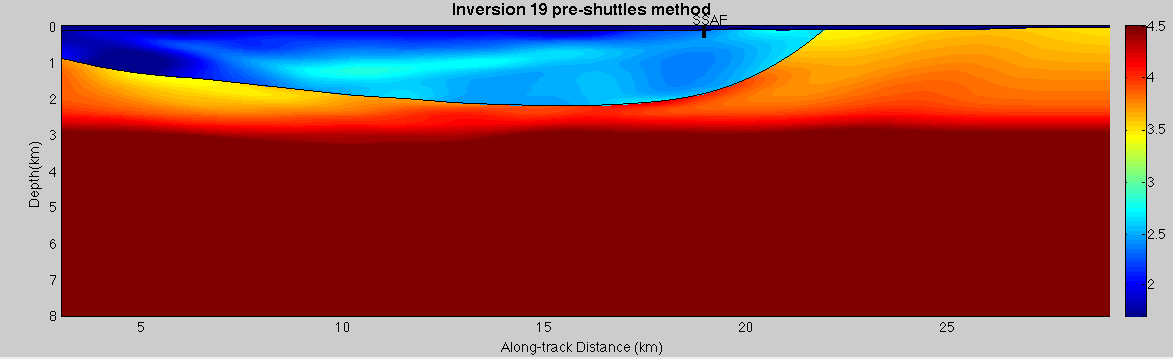
\includegraphics[scale=0.4,keepaspectratio=true]{figs/inv20_preshut.png}
\caption{Inversion 20, inversion iteration 5, velocity model 6.  Chi sq = 6.2895.  The velocity model pre-shuttles method.}
\label{fig:inv20preshut}
\end{figure} 

\begin{figure}[h!]
\raggedleft
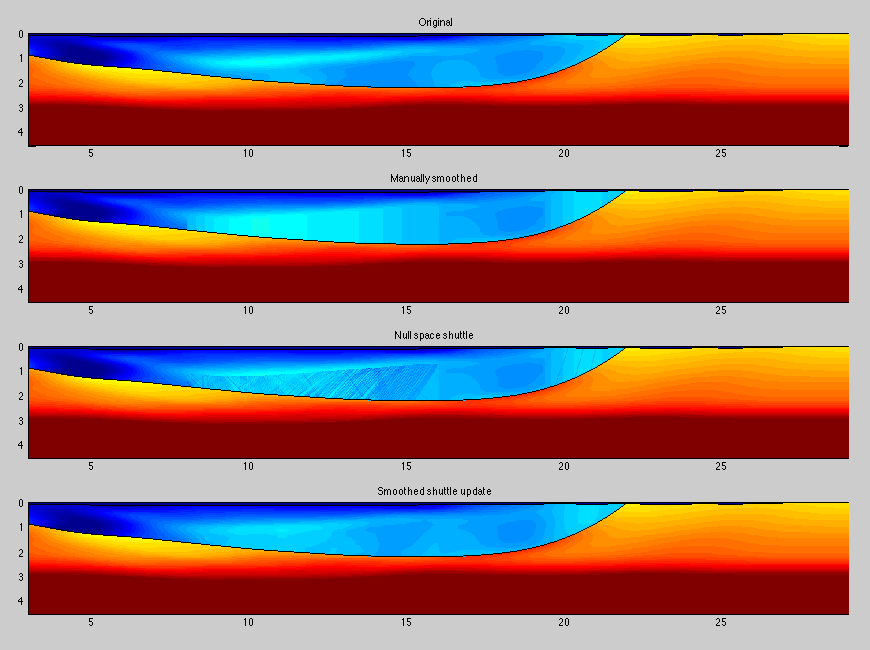
\includegraphics[scale=0.4,keepaspectratio=true]{figs/inv20_postshuttle.png}
\caption{Inversion 20, post shuttle method.  Colorbar is the same as other figures, going from 1.7 km/s to 4.5 km/s.}
\label{fig:inv20postshut}
\end{figure} 

\subexperiment{Inversion 20 Results}
I take the final model to be inversion iteration 15 (velocity model 16), with the best misfit, chi sq = 1.8761.  This model is a still a little "splotchy", but has fewer artifacts than inversion 17's final model and a better misfit.  The final model is in \autoref{fig:inv20final}, and the ray paths and residuals are in \autoref{fig:inv20finalray}.

The low velocity patch around 16 - 21km is still present, and transitions to higher velocities around 21 km along-track distance. 

\begin{figure}[h!]
\raggedleft
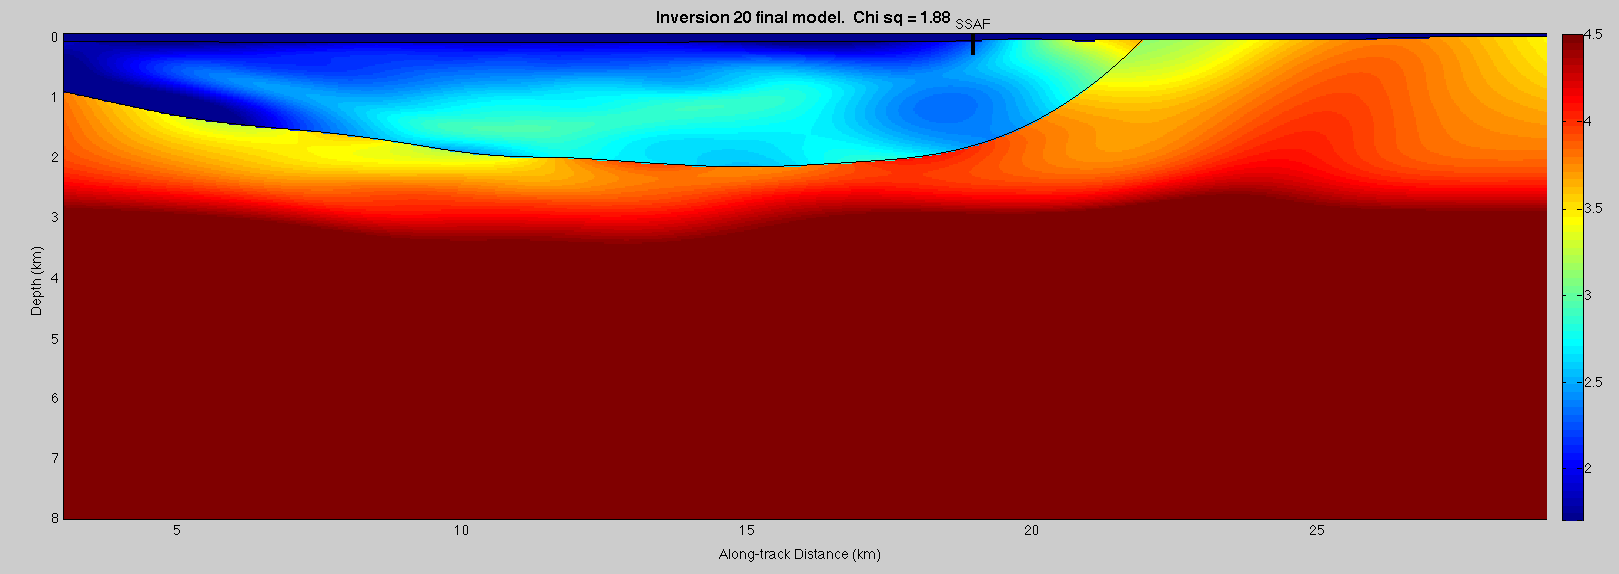
\includegraphics[scale=0.3,keepaspectratio=true]{figs/inv20final.png}
\caption{Inversion 20, final model.  Inversion iteration 15, velocity model 6.  Chi sq = 1.88.}
\label{fig:inv20final}
\end{figure} 

\begin{figure}[h!]
\raggedleft
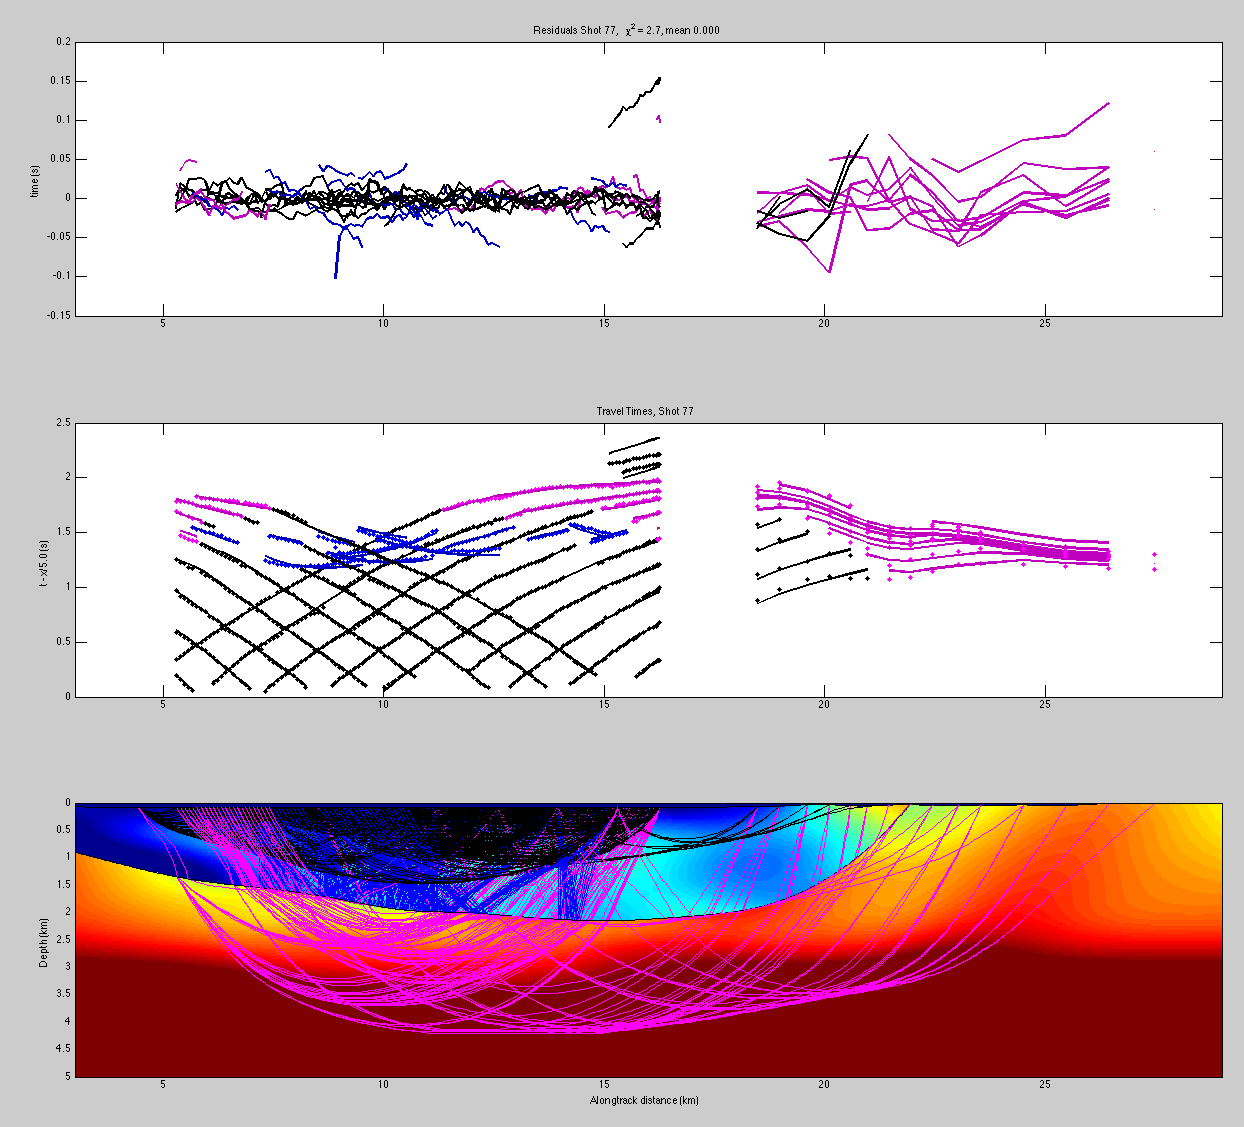
\includegraphics[scale=0.3,keepaspectratio=true]{figs/inv20finalRay.png}
\caption{Inversion 20, final model, ray paths and residuals. Colorbar is the same as in all other figures.}
\label{fig:inv20finalray}
\end{figure} 

\clearpage{}


%-------------------------------Inversion21--------------------------------------------------------
\experiment{Inversion 21 - Inversion 18 w/o MCS constraints}
In here, I run a separate inversion of 18's starting model, without using MCS constraints.

\subexperiment{Inversion 21 Setup}
I copy inversion 18's starting model into the inversion21 directory; I rename it to salton7base\_21\_0.vm.

I copy inversion 18's raytracing and inversion shell scripts, and rename them salton7base\_raytr21.csh and salton7base\_inv21.csh, respectively.

I do not want to constrain the interface location with MCS reflection times, so in the raytracing script I set append = 0.   

All the other parameters remain the same as inversion 18.  

The starting model is the same as inversion18's, and so can be seen in \autoref{fig:inv18start}

\subexperiment{Raytracing and Inversion Output}
Output in \autoref{tab:r21} and \autoref{tab:i21}.

 %Raytracing Output, Inversion 21
\begin{table}[!ht]
\label{tab:r21}
\raggedleft
\begin{tabular}{c l l l l l}
\toprule
\textbf{Raytr, It = } & \textbf{tmean} & \textbf{trms} & \textbf{chi sq} & \textbf{chi r} & \textbf{meanErr} \\
\toprule
It0 & -0.0435 & 0.1321 & 92.0438 & 69.1595 & 0.0152\\
It1 & 0.0113 & 0.1111 & 43.9665 & 45.8497 & 0.0152\\
It2 & 0.0041 & 0.0887 & 26.6384 & 27.2143 & 0.0152\\
It3 & 0.0063 & 0.0712 & 17.2119 & 17.7273 & 0.0152\\
It4 & 0.0053 & 0.0622 & 12.4187 & 12.7683 & 0.0152\\
It5\_orig & 0.0020 & 0.0501 & 8.3514 & 8.4667 & 0.0152\\
It5 & 0.0069 & 0.0711 & 13.9968 & 14.5312 & 0.0152\\
It6 & 0.0020 & 0.0501 & 8.6722 & 8.7863 & 0.0152\\
It7 & -1.7766e-04 & 0.0435 & 6.0834 & 6.0732 & 0.0152\\
It8 & -8.4956e-04 & 0.0360 & 4.4337 & 4.3947 & 0.0152\\
It9 & -0.0025 & 0.0315 & 3.3912 & 3.2751 & 0.0152\\
It10 & -0.0014 & 0.0295 & 2.9143 & 2.8602 & 0.0152\\
It11 & -0.0025 & 0.0260 & 2.3574 & 2.2778 & 0.0152\\
It12 & -9.9098e-04 & 0.0250 & 2.0713 & 2.0486 & 0.0152\\
It13 & -7.7869e-04 & 0.0246 & 1.9692 & 1.9565 & 0.0152\\
It14 & -3.8399e-04 & 0.0246 & 1.9213 & 1.9161 & 0.0152\\
It15 & -6.0576e-04 & 0.0240 & 1.8804 & 1.8739 & 0.0152\\
It16 & -6.4310e-04 & 0.0236 & 1.7967 & 1.7894 & 0.0152\\
It17 & -5.7020e-04 & 0.0242 & 1.8856 & 1.8805 & 0.0152\\
\bottomrule\\
\end{tabular}
\caption{Inversion 21: Raytracing outputs.}
\end{table}

%Inversion Output, Inversion 21
%Inv it 
\begin{table}[!ht]
\label{tab:i21}
\raggedleft
\begin{tabular}{c l l l}
\toprule
\textbf{Inv, It = } & \textbf{set chi sq =} & \textbf{out chi sq =} & \textbf{Penalty} \\
\toprule
It0 & 40 & 41.952 & 14072.16\\
It1 & 25 & 26.226 & 15913.26\\
It2 & 17 & 16.726 & 15878.74\\
It3 & 12 & 12.221 & 15053.86\\
It4 & 8 & 8.0967 & 19587.86\\
It5 & 8 & 8.1305 & 20655.54\\
It6 & 6 & 6.0130 & 21002.41\\
It7 & 4 & 4.0702 & 25407.77\\
It8 & 3 & 2.9995 & 29351.58\\
It9 & 2.5 & 2.4723 & 28122.16\\
It10 & 2 & 2.0019 & 33306.32\\
It11 & 1.8 & 1.8569 & 30866.71\\
It12 & 1.8 & 1.8307 & 27351.31\\
It13 & 1.8 & 1.8273 & 25003.34\\
It14 & 1.8 & 1.7573 & 24597.83\\
It15 & 1.8 & 1.7368 & 23738.40\\
It16 & 1.8 & 1.8179 & 21112.01\\
\bottomrule\\
\end{tabular}
\caption{Inversion 21: Inversion outputs.}
\end{table}

\clearpage{}

\subexperiment{Inversion 21 Shuttles Method}
I apply the shuttles method to inversion iteration 4, velocity model 5.  The original model is in \autoref{fig:inv21preshut} and the shuttled model is in \autoref{fig:inv21postshut}.

\begin{figure}[h!]
\raggedleft
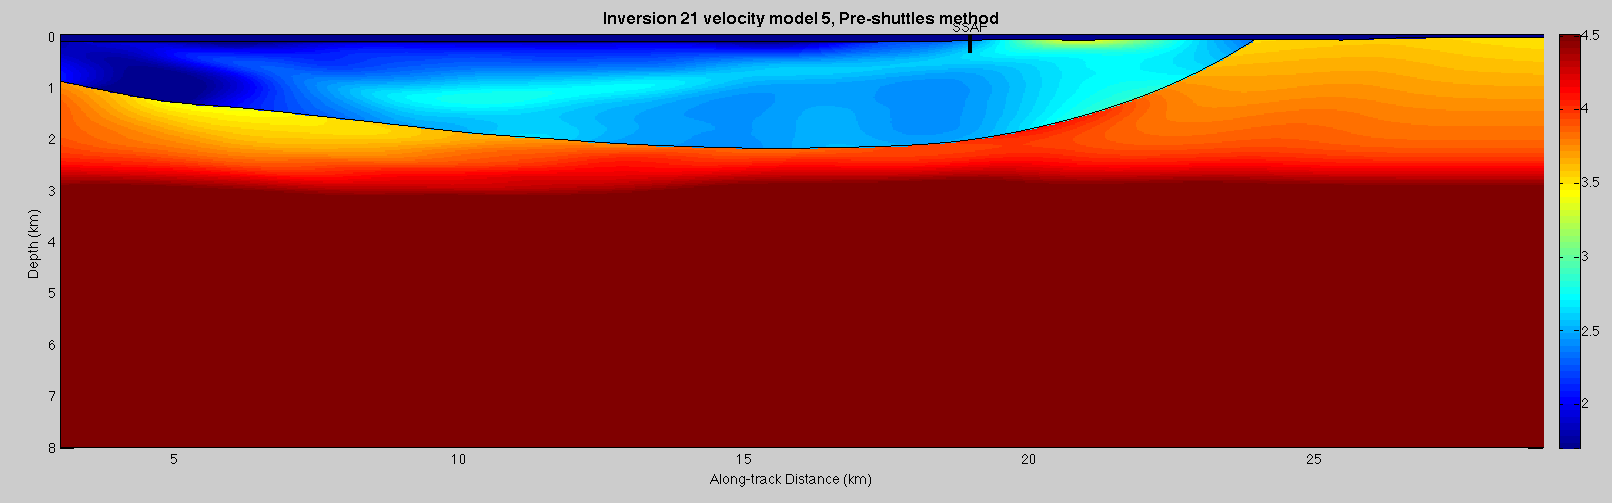
\includegraphics[scale=0.3,keepaspectratio=true]{figs/inv21_preshut.png}
\caption{Inversion 21, pre-shuttles method.  Chi sq = 8.35.}
\label{fig:inv21preshut}
\end{figure} 

\begin{figure}[h!]
\raggedleft
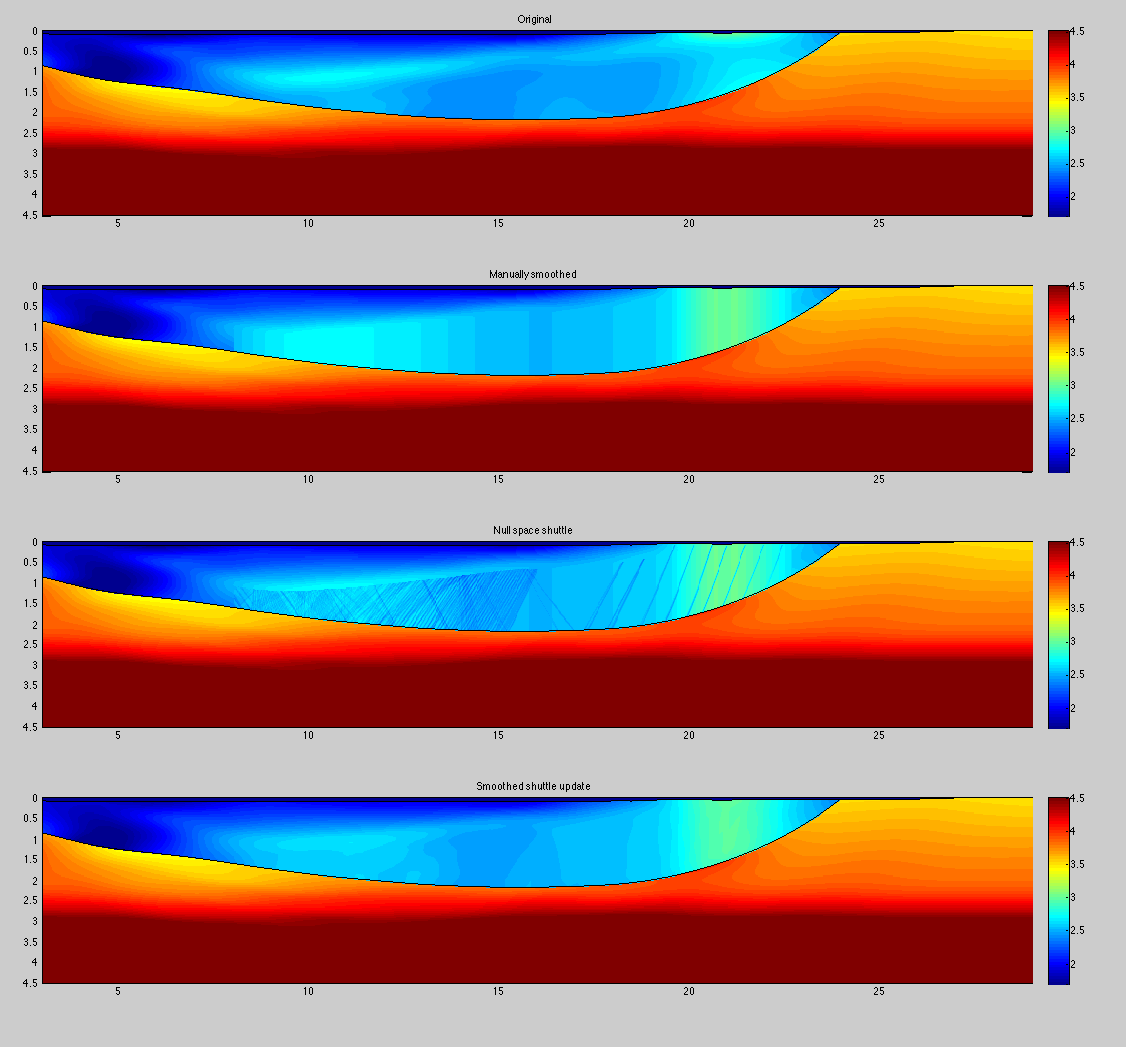
\includegraphics[scale=0.3,keepaspectratio=true]{figs/inv21_postshut.png}
\caption{Inversion 21, post-shuttles method.  Chi sq = 13.99.}
\label{fig:inv21postshut}
\end{figure} 

I use the script salton7\_shuttle\_update.m, and the output shuttled model is in salton\_smshuttle\_inv21.vm.  I copy this into the inversion21 directory; I rename all iteration 5 files to \_orig, and rename the shuttled velocity model to salton7base\_21\_5.vm.  I then ray trace through it.  The statistics for raytracing through the original iteration 5 are in the table as It5\_orig, and through the shuttled model is It5.  


\subexperiment{Inversion 21 Results}
I choose inversion iteration 15, velocity model 16, as the final model.  This had the lowest misfit and did not look splotchier than the other iterations.  The final model is in \autoref{fig:inv21final}, and the ray paths and residuals in \autoref{fig:inv21finalray}.

\begin{figure}[h!]
\raggedleft
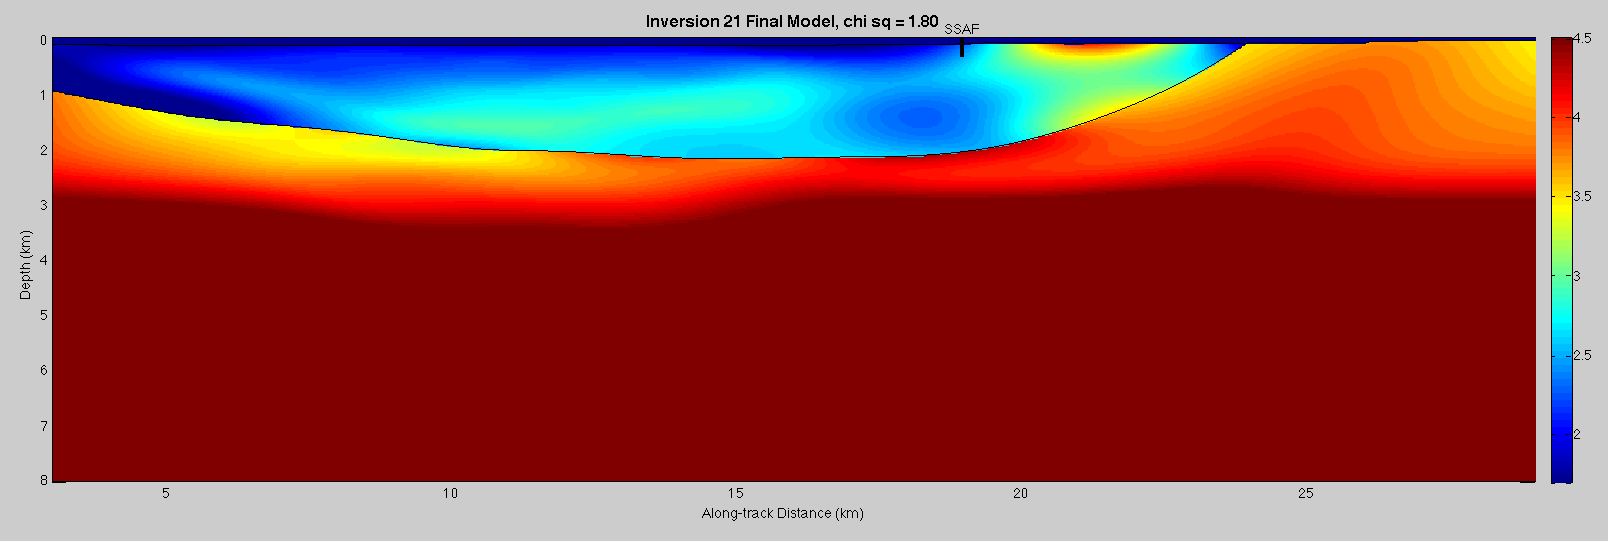
\includegraphics[scale=0.3,keepaspectratio=true]{figs/inv21final.png}
\caption{Inversion 21, final model.  Inversion iteration 15, velocity model 6.  Chi sq = 1.80.}
\label{fig:inv21final}
\end{figure} 

\begin{figure}[h!]
\raggedleft
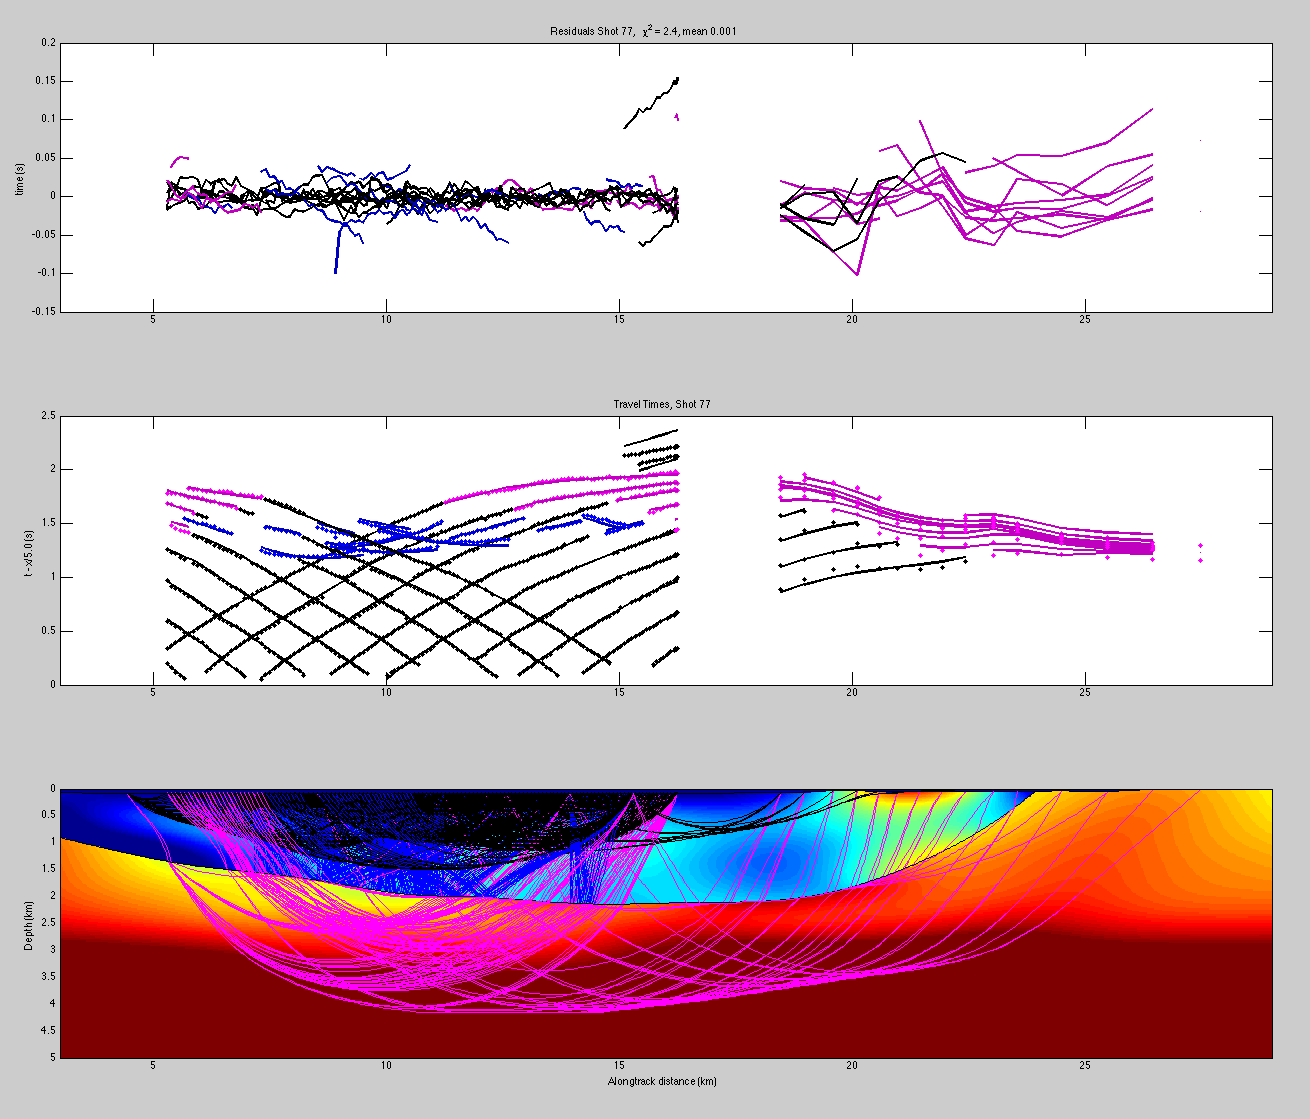
\includegraphics[scale=0.3,keepaspectratio=true]{figs/inv21finalRay.png}
\caption{Inversion 21, final model, ray paths and residuals. Colorbar is the same as in all other figures.}
\label{fig:inv21finalray}
\end{figure} 

\clearpage{}

%----------------------------Summary---------------------------------------
\labday{Thursday, 29 January 2015}
\experiment{Summary}
Summary of the above inversions.  I printed these plots using the script plot\_sfinalint.m.

\subexperiment{Interface at the SSAF surface trace}
Inversion 14 was run at the SSAF trace, and included MCS constraints.  The final model is in \autoref{fig:inv14}.  

\begin{figure}[h!]
\raggedleft
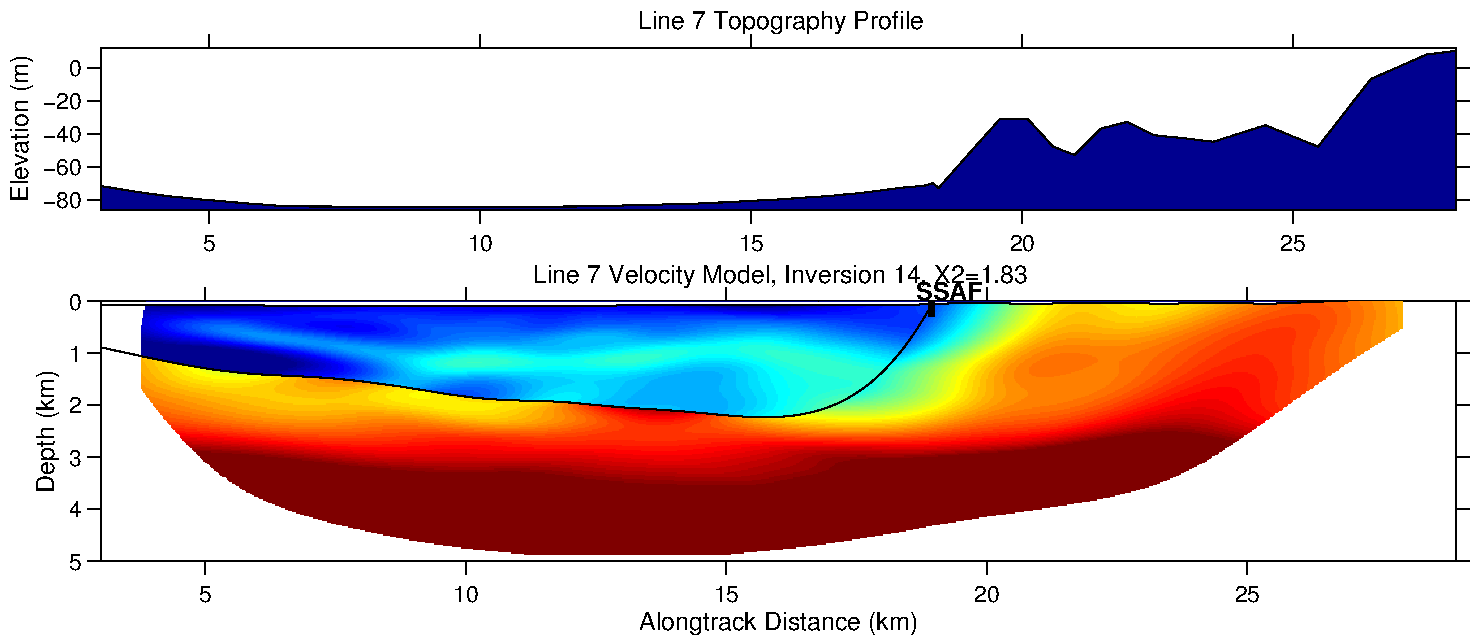
\includegraphics[scale=0.6,keepaspectratio=true]{figs/interface_figures/inv14.pdf}
\caption{Inversion 14, final model plotted with DWS and 1 km ray extension.  $\chi^2 = 1.83$.}
\label{fig:inv14}
\end{figure} 

\subexperiment{Interface to the West of the SSAF surface trace}
There are 2 inversions with the interface intersecting the surface to the west of the SSAF trace: Inversion 15, where it intersects 1 km to the west, and Inversion 16, in which it interests 3 km to the west.  These are seen in \autoref{fig:inv15} and \autoref{fig:inv16}.  In either these two instances, the inversion tries to update velocities that are in layer 2, but adjacent to and to the west of the SSAF, to be slower.  It seems that the best fit would be to move the interface to the east of the SSAF surface trace.

\begin{figure}[h!]
\raggedleft
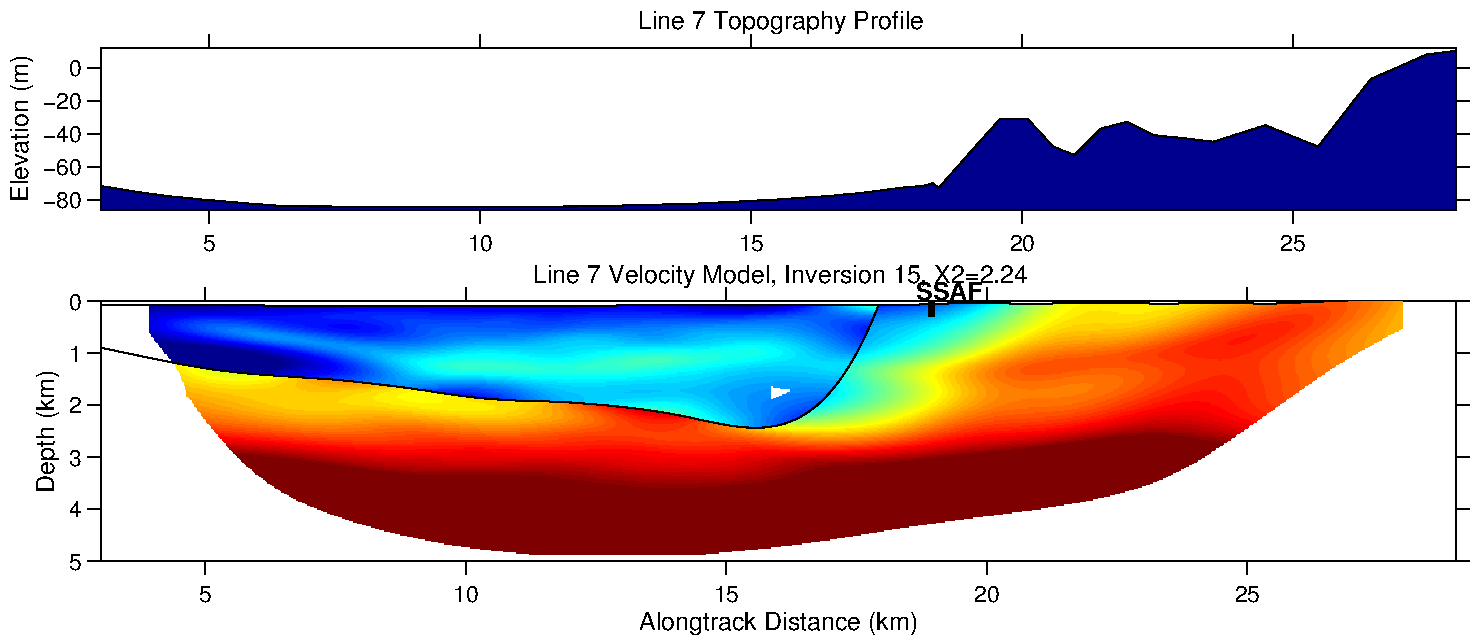
\includegraphics[scale=0.6,keepaspectratio=true]{figs/interface_figures/inv15.pdf}
\caption{Inversion 15, final model plotted with DWS and 1 km ray extension.  $\chi^2 = 2.15$.}
\label{fig:inv15}
\end{figure} 

\begin{figure}[h!]
\raggedleft
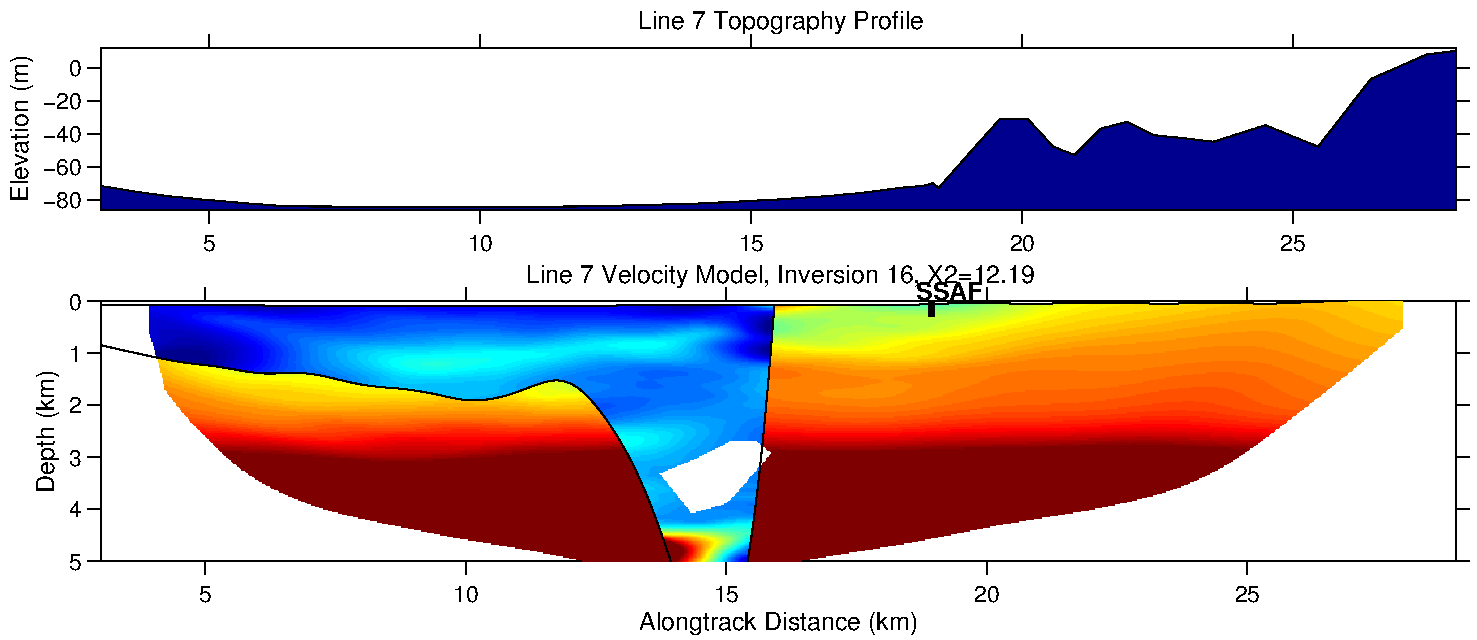
\includegraphics[scale=0.6,keepaspectratio=true]{figs/interface_figures/inv16.pdf}
\caption{Inversion 16, final model plotted with DWS and 1 km ray extension.  $\chi^2 = 12.19$.}
\label{fig:inv16}
\end{figure} 
 
\subexperiment{Interface to the East of the SSAF trace}
There are 4 final inversions with the interface to the east of the SSAF trace: Inversion 17 and 20 (3 km to the east of the SSAF), Inversion 18 and 21 (5 km to the east of the SSAF).  Inversions 17 and 18 use MCS constraints on the interface, and Inversions 20 and 21 do not (Inversion 20 corresponds to 17, and 21 to 18).  Inversions 17 and 20 are plotted in \autoref{fig:inv17} and \autoref{fig:inv20}.  Inversion 20 has a lower misfit than 17; $\chi^2_{17} = 2.07$, and $\chi^2_{20} = 1.88$.  

\begin{figure}[h!]
\raggedleft
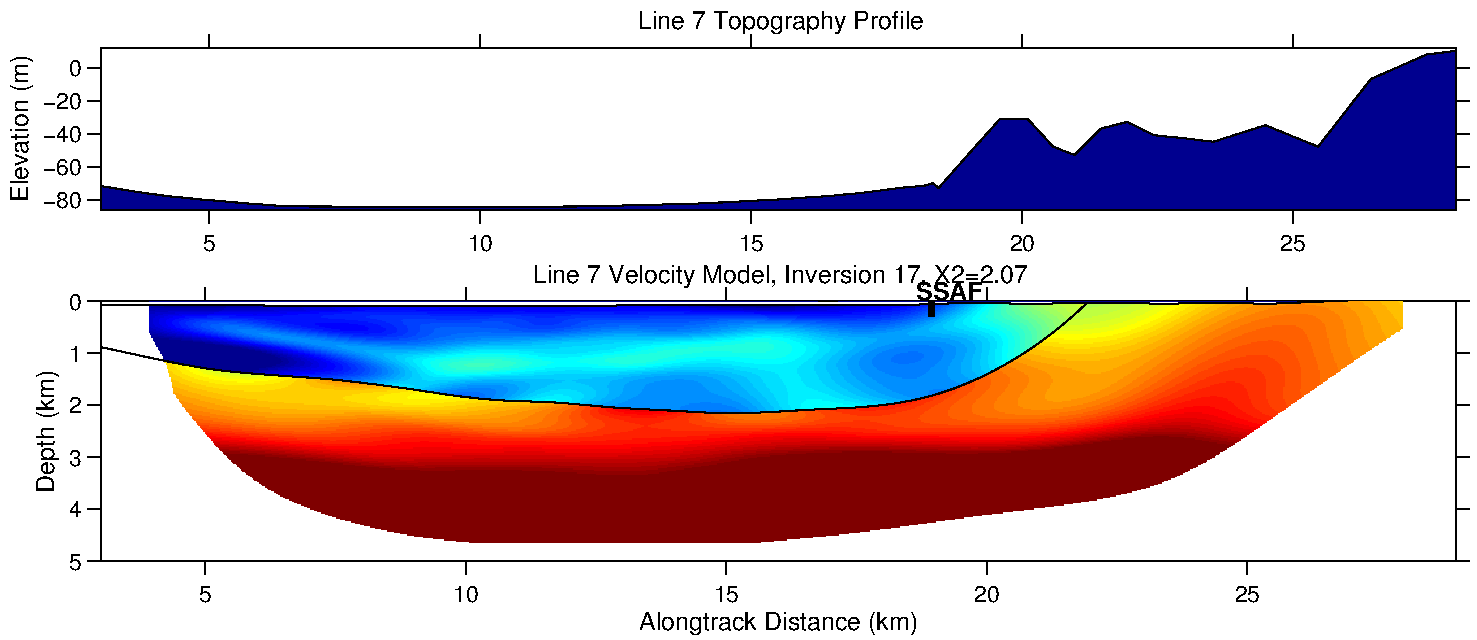
\includegraphics[scale=0.6,keepaspectratio=true]{figs/interface_figures/inv17.pdf}
\caption{Inversion 17, final model plotted with DWS and 1 km ray extension.  $\chi^2 = 2.07$.}
\label{fig:inv17}
\end{figure} 

\begin{figure}[h!]
\raggedleft
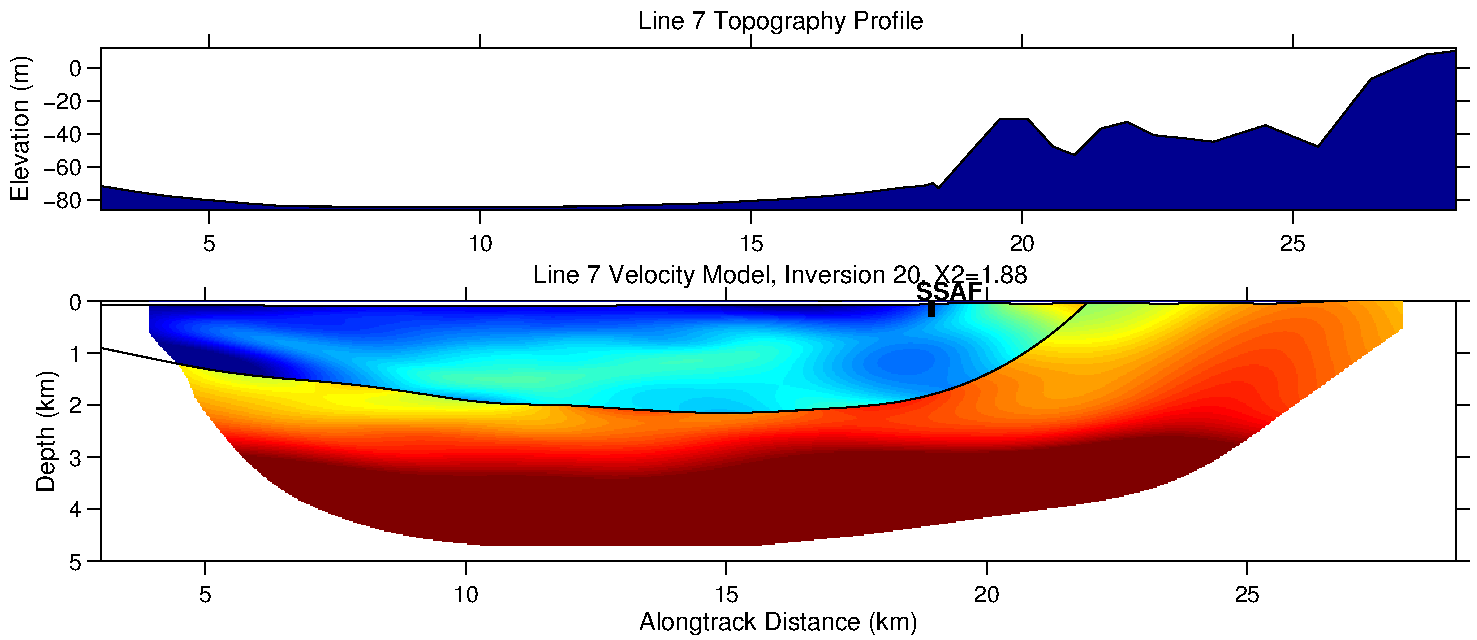
\includegraphics[scale=0.6,keepaspectratio=true]{figs/interface_figures/inv20.pdf}
\caption{Inversion 20, final model plotted with DWS and 1 km ray extension.  $\chi^2 = 1.88$.}
\label{fig:inv20}
\end{figure} 
 
 Inversions 18 and 21 are in \autoref{fig:inv18} and \autoref{fig:inv21}.  These two have the best fit overall: $\chi^2_{18} = 1.90$ and $\chi^2_{21} = 1.80$.  Inversion 21 has a lower misfit and smoother sedimentary basin and high velocity patch, but Inversion 19 also fits the MCS interface constraints (though it has a low velocity "streak" in the basin, and high velocity patches around 20 km along-track distance).  The ray paths and residuals plots for 18 and 21 are seen in \autoref{fig:inv18ray} and \autoref{fig:inv21ray}, respectively. 
 
Because inversion 18 constrains the interface with MCS picks, I take this final model as the "best-fitting" model, and use it for the schematic.  
 
 %velocity models
\begin{figure}[h!]
\raggedleft
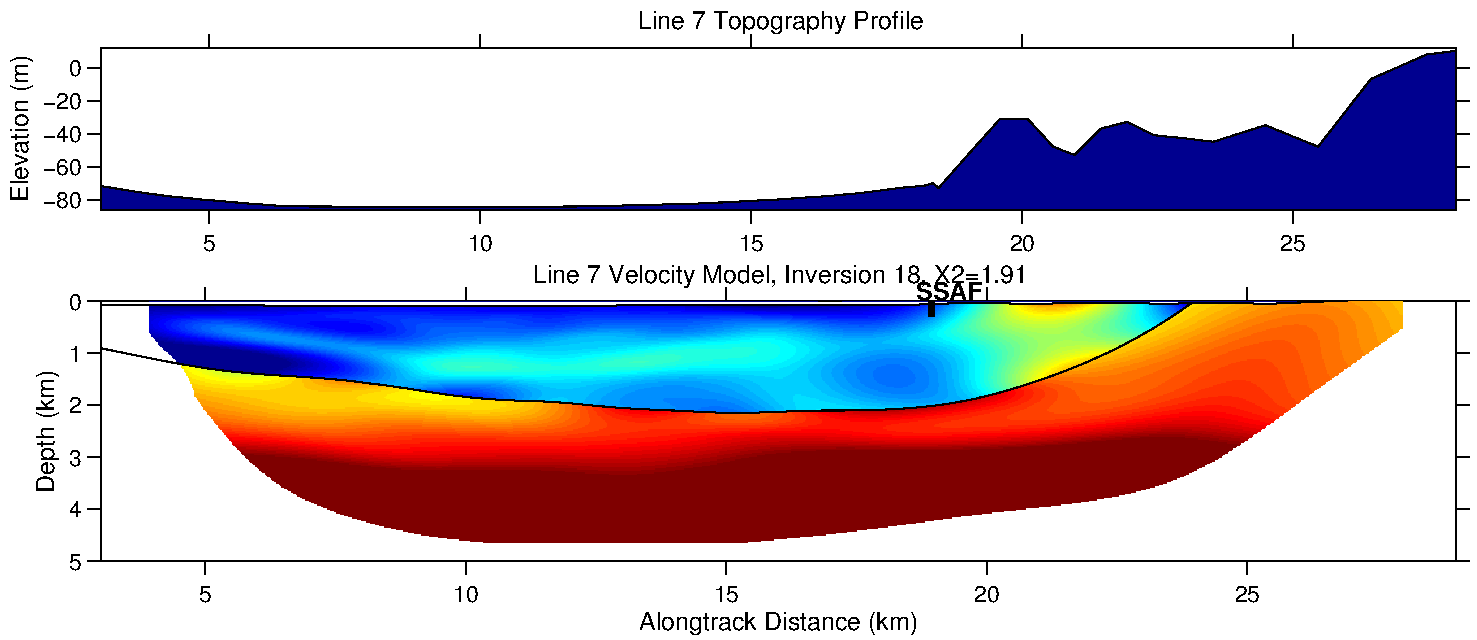
\includegraphics[scale=0.6,keepaspectratio=true]{figs/interface_figures/inv18.pdf}
\caption{Inversion 18, final model plotted with DWS and 1 km ray extension.  $\chi^2 = 1.90$.}
\label{fig:inv18}
\end{figure} 

\begin{figure}[h!]
\raggedleft
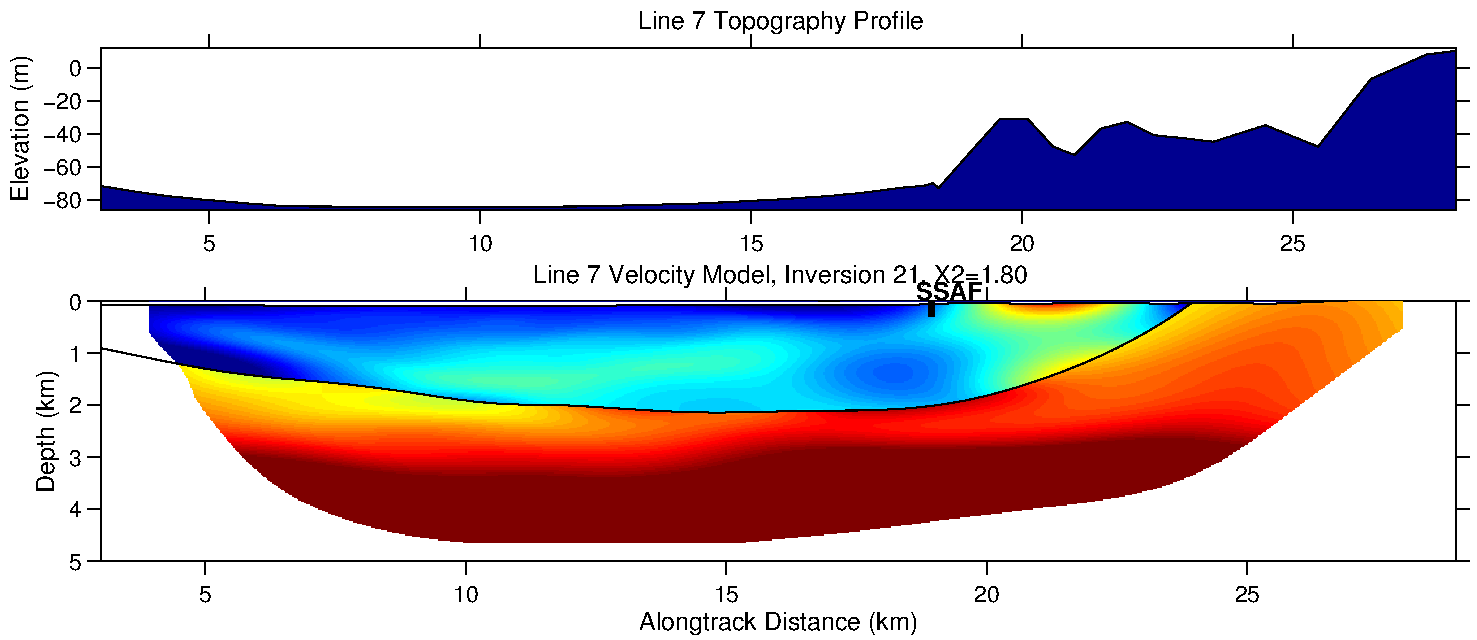
\includegraphics[scale=0.6,keepaspectratio=true]{figs/interface_figures/inv21.pdf}
\caption{Inversion 21, final model plotted with DWS and 1 km ray extension.  $\chi^2 = 1.80$.}
\label{fig:inv21}
\end{figure}
 
 %RAypaths and residuals
\begin{figure}[h!]
\raggedleft
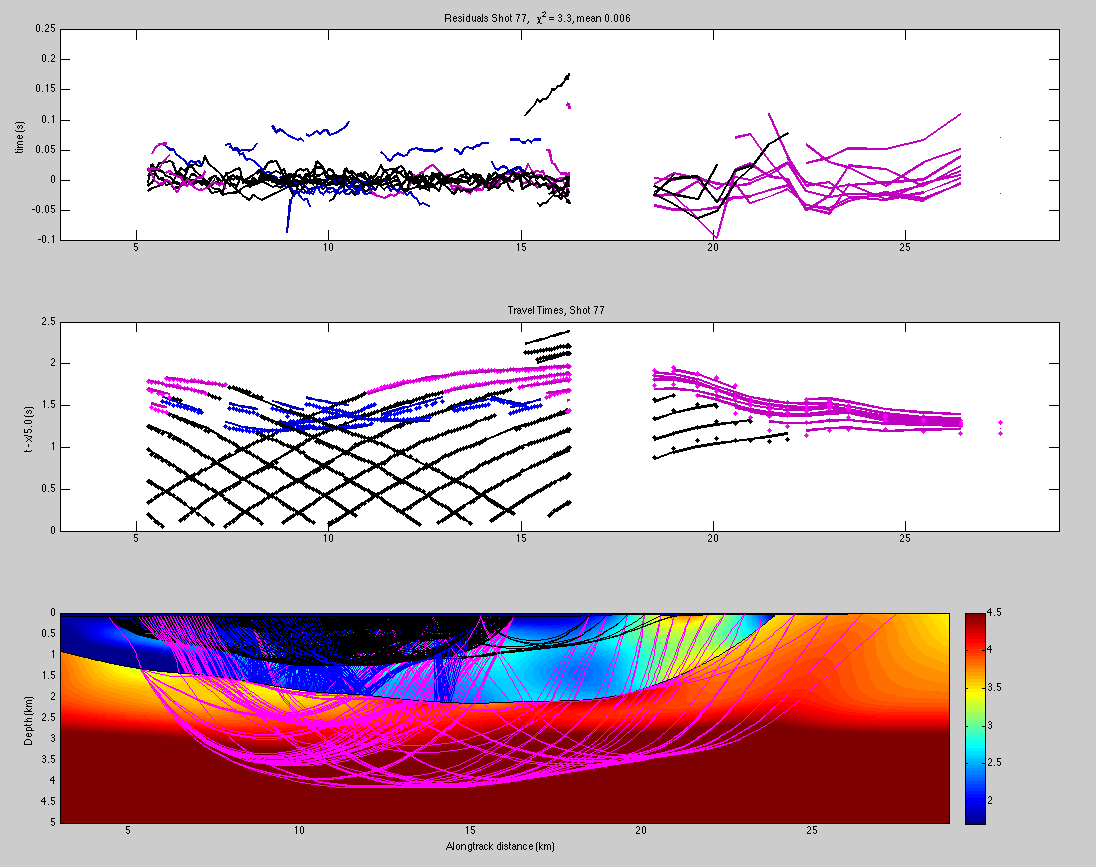
\includegraphics[scale=0.45,keepaspectratio=true]{figs/inv18finalRay.png}
\caption{Inversion 18 ray paths and residuals}
\label{fig:inv18ray}
\end{figure}

\begin{figure}[h!]
\raggedleft
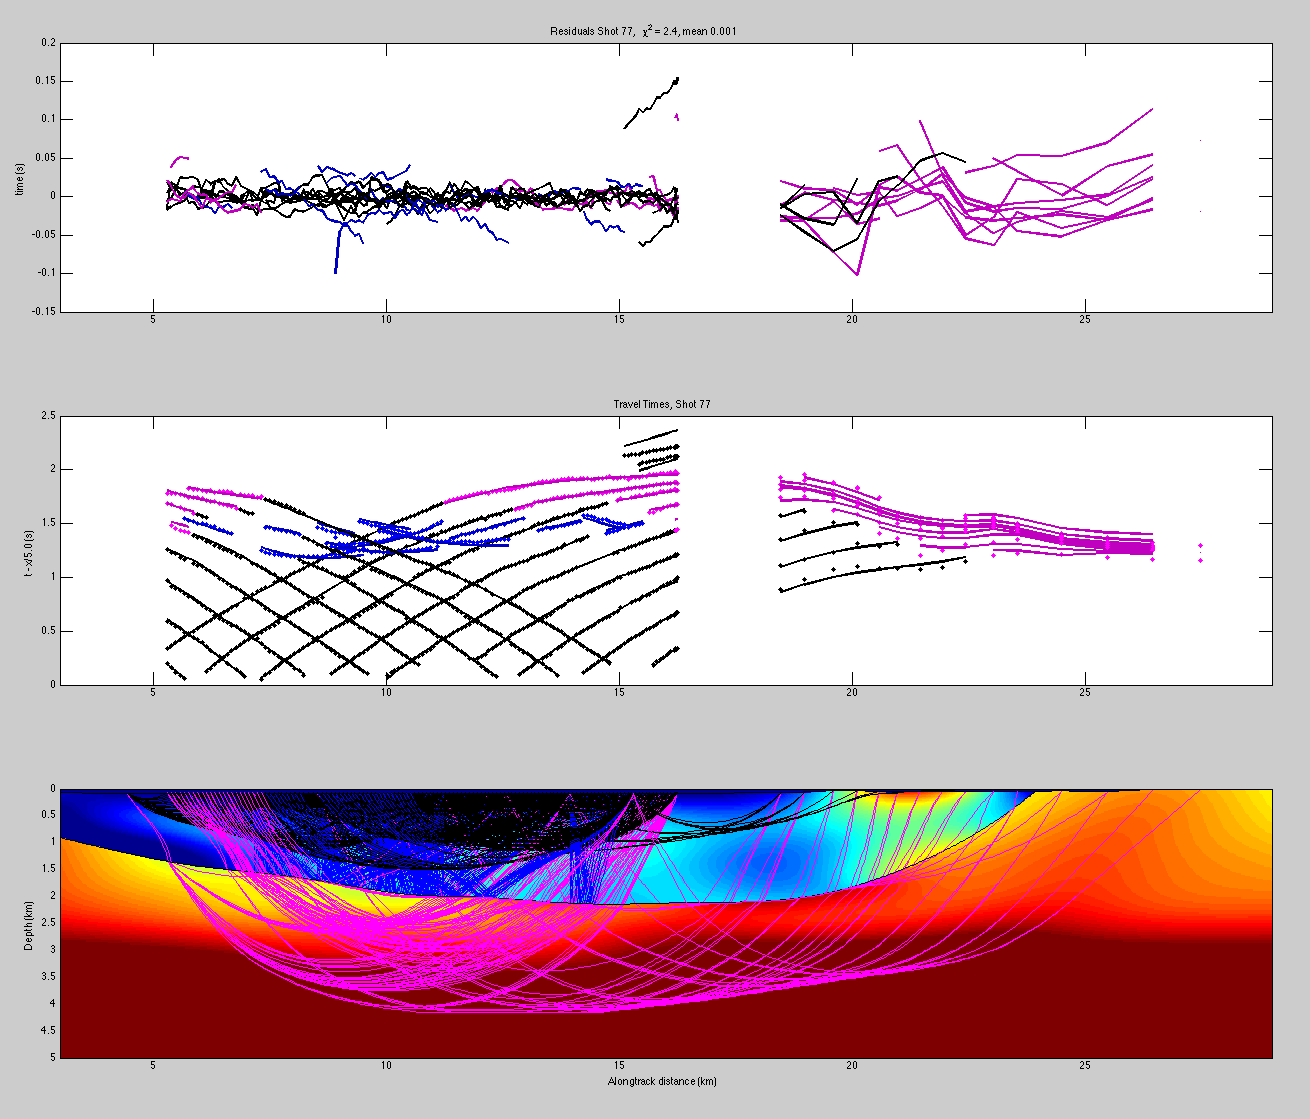
\includegraphics[scale=0.3,keepaspectratio=true]{figs/inv21finalRay.png}
\caption{Inversion 21 ray paths and residuals}
\label{fig:inv21ray}
\end{figure}
 
\subexperiment{Conclusions??}
The current hypothesis (providing I have not overlooked anything with the velocity models) derives its foundation from two main lines of evidence: 

1) The velocity model.  There appears to be a sedimentary wedge, reflecting compacted lake sediments that spatially converge with the dipping reflectors in the sea.  To the east of this, there is a small patch of low-velocities, and further to the east of this the velocities must increase.  

2) Mapped folds from Babcock, 1974.  He observes intense folding between the SSAF and the Salton Sea shoreline; the westernmost layers dip to the west, and the easternmost layers dip into the SSAF.

Because of these two observations, we suggest that the low velocities in the sea are in fact from lake sediments.  The low velocity zone ends approximately near the SSAF surface trace, about 1 km to the east (I'm not sure how well the lateral extent of this can be constrained).  This is likely a damaged zone, which is evident on the surface from the folding that Babcock observes.  The folding is probably caused by a left jog in the SSAF (which also creates uplift at Durmid Hills).  The layers in the west that dip to the west may fall into a transtensional, slightly-westward dipping fault that surfaces in the Salton Sea.  

This hypothesis is illustrated by the schematic in \autoref{fig:cartoon}.

\begin{figure}[h!]
\raggedleft
\includegraphics[scale=0.55,keepaspectratio=true]{/Users/vjsahakian/SaltonSea/Paper/Draft4/figs/schematic/line7schematic_crop.pdf}
\caption{Schematic illustrating the current hypothesis.  The green line denotes the basement reflector observed in the MCS data; between the transtensional fault and the SSAF, folds in solid represent the approximate representation of Babcock's mapped folds, and the dashed lines are an interpretation of how they relate to the greater system.}
\label{fig:cartoon}
\end{figure}
 
\end{addmargin}

%----------------------------------------------------------------------------------------
%	BIBLIOGRAPHY
%----------------------------------------------------------------------------------------

\begin{thebibliography}{9}

\bibitem{lamport94}
Leslie Lamport,
\emph{\LaTeX: A Document Preparation System}.
Addison Wesley, Massachusetts,
2nd Edition,
1994.

\end{thebibliography}

%----------------------------------------------------------------------------------------

\end{document}